\documentclass[a4paper,12pt]{article}
    \usepackage[acronym,toc]{glossaries}
    \usepackage{graphicx} % For figures later
    \usepackage[utf8]{inputenc}
    \usepackage{mathptmx}
    \usepackage{titling}
    \usepackage{comment}
    \graphicspath{ {../images/} }
    \usepackage{caption}
    % SQL tables
    \usepackage{listings}
    \usepackage{float}
    \usepackage{enumerate}% http://ctan.org/pkg/enumerate
    \usepackage[titletoc]{appendix}
    \usepackage{array}
    \newcolumntype{L}[1]{>{\raggedright\let\newline\\\arraybackslash\hspace{0pt}}m{#1}}
    \newcolumntype{C}[1]{>{\centering\let\newline\\\arraybackslash\hspace{0pt}}m{#1}}
    \newcolumntype{R}[1]{>{\raggedleft\let\newline\\\arraybackslash\hspace{0pt}}m{#1}}
    \usepackage{tikz}
    \def\checkmark{\tikz\fill[scale=0.4](0,.35) -- (.25,0) -- (1,.7) -- (.25,.15) -- cycle;} 
    \usepackage{url}
    \usepackage{subfig}
    \usepackage[lithuanian,english]{babel}
    \usepackage[T1]{fontenc}
    
    \makeglossaries
    
    \newglossaryentry{mysql}
    {
        name=MySQL,
        description={ is an open-source relational database management system }
    } 
    \newglossaryentry{docker}
    {
        name=Docker,
        description={  Docker provides an additional layer of abstraction and automation of operating-system-level virtualization on Windows, Linux and MacOS }
    }  
    \newglossaryentry{scala}
    {
        name=Scala,
        description={ Scala is a general-purpose programming language providing support for functional programming and a strong static type system }
    }   
	 \newglossaryentry{seimas}
	{
		name=Seimas,
		description={ The Seimas of the Republic of Lithuania, or simply the Seimas is the unicameral parliament of Lithuania. The Seimas constitutes the legislative branch of government in Lithuania, enacting laws and amendments to the Constitution, passing the budget, confirming the Prime Minister and the Government and controlling their activities }
	} 
   \newglossaryentry{lrs_open}
	{
		name=LRS open data,
		description={ Open data of Lietuvos Respublikos Seimas}
	}   
   \newglossaryentry{k-means}
	{
		name=\textit{k-means},
		description={ }
	} 
   \newglossaryentry{dissimilarity_matrix}
	{
		name=dissimilarity matrix,
		description={ }
	} 
   \newglossaryentry{atviras_seimas}
	{
		name=atviras-seimas.lt,
		description={ }
	} 
   \newglossaryentry{drawio}
	{
		name=draw.io,
		description={ }
	} 
  \newglossaryentry{http}
{
	name=HTTP,
	description={ }
} 
   \newglossaryentry{euclidian}
{
	name=Euclidian distance,
	description={ }
} 
   \newglossaryentry{jvm}
{
	name=JVM,
	description={ }
} 
\newglossaryentry{mockup}
{name={Mockup},description={description}}


    
    % TODO check this list
    \newacronym{api}{API}{Application programming interface}
    \newacronym{auc}{AUC}{ Area under the curve }
    \newacronym{roc}{ROC}{ Receiver operating characteristic }
    \newacronym{hdd}{HDD}{ Hard disk drive }
    \newacronym{csv}{CSV}{ Comma-separated values}
    \newacronym{ip}{IP}{ Internet protocol address }
    \newacronym{tfidf}{TFIDF}{ Term Frequency Inverse Document Frequency }
    \newacronym{io}{IO}{ Input/Output }
    \newacronym{mds}{MDS}{ Multidimensional scaling}
    \newacronym{lrs}{LRS}{ Parliament of the Republic of Lithuania } 
    \newacronym{xml}{XML}{ PLACEHOLDER }   
    \newacronym{sql}{SQL}{  Structured Query Language }   
    
    \begin{document}
   	\selectlanguage{english}
   
    
    \pagenumbering{roman}
    
    \begin{center}
        \section*{Abstract}
    \end{center}
	
        
        \addcontentsline{toc}{section}{\numberline{}\kern-1.5emAbstract}
        
        In Republic of Lithuania, public elects their representatives to a parliament in which new legislation is considered. Due nature of politics, a problem arises once citizens wants to observe and evaluate parliament members work. Main output of parliament is their votes for various legislatures. Voting data is publicly available through \gls{lrs} website. This project aims to visualize voting patterns and their changes. Another goal is to provide public access to results.
        
        In the project \gls{mds} and \gls{k-means} clustering are used to analyze voting patterns. Software to download, process and visualize  data is written with \gls{scala}.
        

    \clearpage
    
    \begin{center}
    	\section*{Santrauka}
    \end{center}
    
    
   	\addcontentsline{toc}{section}{\numberline{}\kern-1.5emSantrauka}
    \begin{otherlanguage}{lithuanian}
    	Atstovus į Lietuvos Respublikos Seimą (LRS), kuriame yra apsvarstomi ir priimami nauji įstatymai, išrenka Lietuvos piliečiai. Tačiau iškyla problemų visuomenei norint iš arčiau stebėti ir įvertinti Seimo narių darbą. Viena pagrindinių Seimo narių pareigų ir yra balsavimas priimant įvairius naujus įstatymus ar jų pataisymus. Kiekvieno Seimo nario balsai yra viešai prieinami Lietuvos Respublikos Seimo internetinėje svetainėje. Šiuo darbu siekiama šią informaciją vizualizuoti, kad būtų galima stebėti balsavimo modelius ir jų pasikeitimus. Taip pat yra siekiama suteikti viešą prieigą prie šių rezultatų.
    	
    	Darbe, analizuojant balsavimo modelius, yra naudojamas daugiadimencinis skalių metodas ir k-reikšmių klasterizacija. Programinė įranga, duomenų atsisiuntimas ir vizualizavimas yra parašytas naudojantis Scala.
    	
    \end{otherlanguage}

	\clearpage

    \tableofcontents
    
    \clearpage
    
    \printglossary[type=\acronymtype]
    
    \printglossary
    
    \clearpage
    
    \pagenumbering{arabic}
    
    \section{Introduction}
    
    In Republic of Lithuania, public elects their representatives to a parliament in which new legislation is considered. By this election each citizen delegates specifics of legislation process to their representatives so they don't have to actively participate in the process.
	
	However, a problem arises once citizen wants to validate what his representative has been doing. Single term of office NEEDS-CITATION involves thousands of complicated laws and votes. To analyze everything becomes almost an impossible task for a single citizen who is out of the loop. 
	
	To make it easier there are journalists, politologists and other personas who review new legislation, current issues. Delegates themselves also do press conferences, debates where they state their intentions, comment on their actions. However, this requires citizens to trust that journalists and delegates only state truth, don't omit important information and don't have other hidden agendas. Study done about intrinsic honesty showed that the more society is corrupt - the more people lie in a simple dice game. This applies to politicians too and citizens trust in parliament is relatively low.  Therefore, anything that can be done to better observe representatives is useful.

	This project aims to deliver a software system which can be accessed online with research done available to any user. Research will include visualizations of \acrfull{mds} for specific time periods of a given term. \Gls{k-means} projected on \gls{mds} output to visualize minority vs majority and to see if there are secret groups.
    
    \clearpage
    
    \section{Analysis}
   
   	\subsection{Literature analysis}
   	
	There is a decent amount of previous work analyzing voting on roll call data. A huge part of this research is on specific elections that happened in the past.\\	
	
	In \textit{Spatial Models of Parliamentary Voting} \cite{poole_2005} author discusses how voter's positions on specific issues can be captured by his position on one or two dimensions such as liberalism or conservatism. This constraint means there are two spaces - one with few dimensions - basic  or ideological. The other - high dimensional space which represents remaining issues. This breakthrough might suggest \acrlong{mds} as a good performance method for visualization and analysis as majority of data is encoded in few dimensions.\\
	
	
	There is research done specifically on \gls{lrs} data. One such is \textit{On Structural Analysis of Parliamentarian Voting Data} \cite{DBLP:journals/informaticaLT/KrilaviciusZ08}. In this paper authors discuss about data reduction to \gls{dissimilarity_matrix}, vote encoding, \gls{mds} and its performance on specific dimensions. Authors focus on specific elections and term of office which is different from our goal. However, methods discussed and research results are relevant for this project.\\
	
	Master thesis was written few years ago on \gls{lrs} voting which included similar analysis. One of research areas was to see if there are hidden groups in the parliament \cite{vytautas_mick_magistrinis}. Author was not able to detect hidden groups. In this project, goal, data and parameters are different so conclusion might differ too. Method used was \textit{k-means} clustering and data was showed on \gls{mds} reduced coordinates. In this project similar approach can be taken with different parameters like date ranges for votes.  \\
	
	In \textit{The new Voteview.com: preserving and continuing Keith Poole’s infrastructure for scholars, students and observers of Congress} \cite{article} paper, authors discuss famous \textit{Voteview.com} website. While website's primary goal is to provide open data access is different from ours - it contains useful information about how specific methods are used, how visualizations work. It also contains visualization which shows how data changed over time - how ideology and party composition changes.
	
		
	
	
	\clearpage
	
	\subsection{Materials and methods}
   	
 	\subsubsection{Lithuania's parliament open data semantics analysis }
 	
 	In this section open data from \acrshort{xml} is reviewed. Only data and properties important to the project are included and commented on. All data is imported into \gls{mysql} database, therefore to demonstrate structure tables are used. Field types are inferred empirically by looking at data, therefore might not be correct in some cases. Moreover, data itself is not consistent through all years of \acrlong{lrs} activity.\\
	
	\noindent
	Table \ref{tab:term_of_office} contains term of office table structure.
	\begin{center}
	 	\begin{tabular}{L{3cm} L{3cm} L{2.2cm} L{3.8cm}}
	 		\multicolumn{4}{c}{}\\ 
	 		\hline
	 		In XML & In database & Type & Comments\\
	 		\hline 
	 		kadencijos\_id & term\_of\_office\_id & int(11) & Unique term of office id \\ 
	 		pavadinimas & name & varchar(255) not null & Name \\
	 		data\_nuo & date\_from & date not null & Date when term of office begins \\ 
	 		data\_iki & date\_to & default null & Date when term of office ends \\
	 		\hline
	 	\end{tabular}
	 	\captionof{table}{Term of office table structure} \label{tab:term_of_office}
	\end{center}

	\hfill
	
	
	\noindent
	Table \ref{tab:sessions} contains parliament sessions table structure.
	\begin{center}
		\begin{tabular}{L{3cm} L{3cm} L{2.2cm} L{3.8cm}}
			\multicolumn{4}{c}{}\\ 
			\hline
			In XML & In database & Type & Comments\\
			\hline 
			sesijos\_id & session\_id & int(11) not null & Unique parliament session id \\
			kadencijos\_id & term\_of\_office\_id & int(11) & Unique term of office id \\ 
			numeris & number & varchar(255) not null & Number \\ 
			pavadinimas & name & varchar(255) not null & Session name \\ 
			data\_nuo & date\_from & date not null & Date when session begins \\
			data\_iki & date\_to & date default null & Date when session ends. Current session doesn't have this value set. \\
			\hline
		\end{tabular}
		\captionof{table}{Parliament session table structure} \label{tab:sessions}
	\end{center}
	
	\hfill
	
	\noindent
	Table \ref{tab:plenary} contains parliament plenaries table structure.
	\begin{center}
		\begin{tabular}{L{3cm} L{3cm} L{2.2cm} L{3.8cm}}
			\multicolumn{4}{c}{}\\ 
			\hline
			In XML & In database & Type & Comments\\
			\hline
			posėdžio\_id & plenary\_id & int(11) not null & Unique plenary id \\
			sesijos\_id & session\_id & int(11) not null & Unique parliament session id \\
			numeris & number & varchar(255) not null & Number \\ 
			tipas & plenary\_type & varchar(255) not null & Plenary type \\ 
			pradžia & time\_start & datetime default null & Plenary starting time \\
			pabaiga & time\_finish & datetime default null & Plenary ending time. Some plenaries are not yet finished and some entries don't include times at all \\
			\hline
		\end{tabular}
		\captionof{table}{Plenary table structure} \label{tab:plenary}
	\end{center}
	
	\hfill

	\noindent
	Table \ref{tab:parliament_member} contains parliament member table structure.
	\begin{center}
		\begin{tabular}{L{2.5cm} L{4cm} L{2.2cm} L{3.3cm}}
			\multicolumn{4}{c}{}\\ 
			\hline
			In XML & In database & Type & Comments\\
			\hline
			asmens\_id & person\_id & int(11) not null & Person id\\
			- & unique\_id & varchar(100) not null & Unique id for person, generated by script\\
			vardas & person\_name & varchar(255) not null & Member name \\
			pavardė & person\_surname & varchar(255) not null & Member surname \\
			lytis & gender & varchar(1) not null & Gender \\
			data\_nuo & date\_from & date not null & Date from inauguration\\
			data\_iki & date\_to & date default null & Date when term ends. Current session doesn't have this value set. \\
			iškėlusi\_partija & faction\_name & text & Faction name \\
			išrinkimo\_būdas & elected\_how & varchar(255) not null & How member was elected\\
			biografijos\_nuoroda & biography\_link & varchar(255) default null & Hyperlink to biography\\
			- & term\_of\_office\_id & int(11) & Unique term of office id \\
			- & term\_of\_office\_specific\_id & int(11) & Specific term id used for computations \\
			- &	faction\_id & int(11) not null & Faction id \\
			\hline
		\end{tabular}
		\captionof{table}{Parliament member table structure} \label{tab:parliament_member}
	\end{center}
	
	\hfill
	
	\noindent
	Table \ref{tab:agenda_question} contains agenda question table structure.
	\begin{center}
		\begin{tabular}{L{3cm} L{4.2cm} L{3cm} L{2.5cm}}
			\multicolumn{4}{c}{}\\ 
			\hline
			In XML & In database & Type & Comments\\
			\hline
			darbotvarkės\_klausimo\_id & agenda\_question\_id & int(11) not null & Agenda question id\\
			- & agenda\_question\_group\_id & varchar(255) not null & Group id\\
			pavadinimas & title & text & Title \\
			laikas\_nuo & time\_from & time default null &  Question start time \\
			laikas\_iki & time\_to & time default null & Question end time \\
			- & datetime\_from & datetime default null & Custom generated date time \\
			- & datetime\_to & datetime default null & Custom generated date time\\
			data & date &  date not null & Date\\
			pavadinimas & raw\_status & varchar(255) not null & Status as taken from XML \\
			- & status & int(5) default null & Status encoded \\
			dokumento\_nuoroda & document\_link & varchar(255) default null & Hyperlink to document\\
			- & speakers & text & Speakers list converted from XML to single text field with separators \\
			numeris & number & varchar(255) not null & Number \\
			- & plenary\_id & int(11) not null & Plenary id\\			                                    
			\hline
		\end{tabular}
		\captionof{table}{Agenda question table structure} \label{tab:agenda_question}
	\end{center}
	
	\hfill
	
	\noindent
	Table \ref{tab:plenary_question} contains plenary question table structure.
	\begin{center}
		\begin{tabular}{L{3cm} L{4.2cm} L{3cm} L{2.5cm}}
			\multicolumn{4}{c}{}\\ 
			\hline
			In XML & In database & Type & Comments\\
			\hline
			darbotvarkės\_klausimo\_id & agenda\_question\_id & int(11) not null & Agenda question id\\
			- & plenary\_question\_group\_id & varchar(255) not null & Group id\\
			pavadinimas & title & text & Title \\
			laikas\_nuo & time\_from & time default null &  Question start time \\
				- & datetime\_from & datetime default null & Custom generated date time \\
			pavadinimas & raw\_status & varchar(255) not null & Status as taken from XML \\
			- & status & int(5) default null & Status encoded \\
			numeris & number & varchar(255) not null & Number \\
			- & plenary\_id & int(11) not null & Plenary id\\				                                    
			\hline
		\end{tabular}
		\captionof{table}{Plenary question table structure} \label{tab:plenary_question}
	\end{center}
	
	\hfill
	
		\noindent
	Table \ref{tab:discussion_events} contains discussion event table structure.
	\begin{center}
		\begin{tabular}{L{3cm} L{4.2cm} L{3cm} L{2.5cm}}
			\multicolumn{4}{c}{}\\ 
			\hline
			In XML & In database & Type & Comments\\
			\hline
			- & agenda\_question\_id & int(11) not null & Agenda question id\\
			- & unique\_id & varchar(255) not null & Custom generated unique id\\
			laikas\_nuo & discusstion\_time\_from & time default null &  Event start time \\
			asmens\_id & person\_id & nt(11) not null & Person id\\
			balsavimo\_id & vote\_id & int(11) not null & Vote id\\
			balsavimo\_tipas & vote\_type & int(5) default null & Vote type \\
			- & plenary\_id & int(11) not null & Plenary id\\				                                    
			\hline
		\end{tabular}
		\captionof{table}{Discussion event table structure} \label{tab:discussion_events}
	\end{center}

	\hfill
	
			\noindent
	Table \ref{tab:vote} contains vote table structure.
	\begin{center}
		\begin{tabular}{L{3cm} L{4.2cm} L{3cm} L{2.5cm}}
			\multicolumn{4}{c}{}\\ 
			\hline
			In XML & In database & Type & Comments\\
			\hline
			- & vote\_person\_id & int(11) not null & Custom generated unique id for vote\\
			balsavimo\_laikas & time & time DEFAULT not null &  Voting time \\
			balsavo & vote\_total & int(11) not null & How many voted\\
			viso & vote\_total\_max & int(11) not null & How many can vote\\
			už & vote\_for & int(11) not null & Voted for\\
			prieš & vote\_against & int(11) not null & Voted against\\
			susilaikė & vote\_abstain & int(11) not null & Voted abstain\\
			komentaras & comment & text & Vote comment\\
			asmens\_id & person\_id & int(11) not null & Person id\\
			asmeyns\_vardas & person\_name &  varchar(255) not null & Person name\\
			asmens\_pavarde & person\_surname &  varchar(255) not null & Person surname\\
			kaip\_balsavo & vote & int(11) not null & Vote itself\\
			- & vote\_person\_id & int(11) not null & Custom generated unique id for vote\\
			frakcija & faction\_acronym & varchar(255) default null & Acronym for faction\\
			balsavimo\_id & vote\_id & int(11) not null & Vote id\\
			balsavimo\_tipas & vote\_type & int(5) default null & Vote type \\
			- & vote\_id & int(11) not null & Vote id\\
			- & plenary\_id & int(11) not null & Plenary id\\				                                    
			\hline
		\end{tabular}
		\captionof{table}{Votes table structure} \label{tab:vote}
	\end{center}
	
	\hfill
	
	\clearpage
	
		\subsection{Method analysis}
	\subsubsection{MDS}
	
	\acrfull{mds} is a method to visualize similarity of individual cases for a specific dataset. It takes an input matrix called proximity matrix $\Upsilon$ (or distance matrix). Proximity matrix is symmetric matrix containing distances between all objects $\psi$. Or in more generic terms - it contains similarities or dissimilarities of pairs. Actual distance can be calculated using Euclidian distance as described in formula \ref{eq:1}. Classic \acrshort{mds} will assume distance to be Euclidian.
	\begin{center}
		\begin{equation}\label{eq:1}
		d(\mathbf{p},\mathbf{q}) = \sqrt{\sum_{i=1}^n (q_i-p_i)^2}
		\end{equation}
	\end{center} 
	
	 Method outputs coordinate matrix minimizes loss function $strain$ \cite{BorgGroenen2005}. Given proximity matrix $\Upsilon$, goal of \acrshort{mds} is to find $\psi$ vectors $q_i,...,q_\psi$ such that $||q_i - q_j\| \approx \upsilon_{ij} \forall i,j \in 1,...,\upsilon$, where $||x||$ is vector norm. 
	
	
	\subsubsection{Unsupervised learning: {\textit k-means} clusterization }
	
%	Due missing labels of this dataset we are forced to look into unsupervised machine learning methods. \textit{k-means} clusterization \cite{clusterization} is one such method and it fits well with our features. This is due \acrshort{tfidf} which transforms text into vectors be used with \textit{k-means}.
%	For distance between comments we can use cosine similarity \cite{cosine_similarity} due its nature of performing better when comparing texts. To compare we can try with Euclidian and Manhattan distances too.
%	

	\gls{k-means} performance can be measured two ways: manually and with \textit{distortion}. It is possible to inspect clusters and see if results given are somewhat correct. \textit{Distortion} is final sum of the squared distances between each vector and its centroid \cite{selection_k_means}.

	\clearpage
	 
 	 
 	\subsection{Problem analysis}
 	
 	Problem can be divided into two pieces:
 	\begin{itemize}
 		\item Research part, including \gls{mds} and \gls{k-means} classification
 		\item Software development
 	\end{itemize}
 	
 	If considered what is output of parliaments during their term of office in parliament - it would be their voting outcomes. Let's say there is a set of all votes made by parliament members $V = \{v_1, v_2, ... v_n\}$ where each vote $v_i$ has a tuple of parameters $P = \{timestamp, term\; of\; office, parliament\;member\;id, voting\;outcome,...\}$. Votes can be divided into groups depended on term of office $T$ during which they were cast. Each term of office $T_i$ can be divided into smaller arbitrarily chosen time periods $\{p_1, p_2, ...p_n\}$. Each time periods can have votes assigned which were cast during that time. Goal is visualize set $V$ in a way that similar voting patterns of different members are visible. 
 	
 	In order to visualize voting patterns by members, its dimensions need to be reduced. With help of \acrfull{mds}, vote set $V$ with parameters set $P$ can be visualized on a two or one dimensional coordinate system. As discussed in literature analysis and \cite{poole_2005} voting patterns can be captured by only few dimensions. To observe how voting patterns change during time, different time periods could be chosen. Term of office should be the maximum time period $p_n$ to analyze, as majority and minority usually changes together with parliament members.
 	
 	Another goal is to see if votes can be classified to certain political groups` without knowing who voted. This also enables us to see if there are hidden factions between the explicitly stated ones. As discussed in literature analysis, in order to predict if voting pattern reveals political faction, majority or minority side, different amount of clusters need to be chosen. Finding clusters $\{c_1, c_2,...c_n\}$ representing political faction voting patterns and then assigning votes to the specifics clusters will show how similarly explicitly stated sides vote. 
 
 	
 	\clearpage
 	
 	%
 	% Problemos analizė – nagrinėjamoji problema turi būti atskleista moksliniais ar profesiniais terminais, mokslinėmis hipotezėmis ar techninėmis specifikacijomis. Problemos aktualumas turi būti pagrįstas literatūros ir savarankiška analitine apžvalga. Šioje dalyje:
 	% • Pateikiamos teorinės nuostatos, kurios paaiškina darbe nagrinėjamą problemą;
 	% • Įvertinamas pasirinktos problemos teorinio ištyrimo laipsnis;
 	% • Remiantis literatūros šaltiniais, įvertinami skirtingi atskirų autorių problemos traktavimo variantai ir vyraujantys požiūriai;
 	% • Įvertinami siūlomi literatūroje teoriniai problemos %sprendimo būdai (metodai);
 	% • Pagrindžiama pasirinktos problemos tyrimo logika bei metodai.
 	% Teorinė dalis neturi būti aprašomojo (referato) pobūdžio. Darbo autorius privalo pateikti ir pagrįsti savo asmeninę nuomonę, diskutuoti su kitų tyrinėtojų teiginiais apie sprendžiamą problemą.

    
    \clearpage
    
    \section{Design and development of atviras-seimas.lt}
    \subsection{Components of system}
   	\subsubsection{Functional requirements}
   	
   	Main goal of software is to provide public access for masses to view analysis and research done in this project. Software will run on virtual server and be available online on \gls{atviras_seimas}. There are two main roles: guest user and scientist. Users will be able to access system with any modern browser. Scientist, or the person maintaining project will be able to update data to most recent one on \gls{lrs_open} website.
   
   	
   	 Data is visualized using interactive diagrams. In table \ref{tab:system_features} functional requirements are presented.
   	
 	\noindent
   	\begin{center}
   		\begin{tabular}{L{8cm} C{1cm} C{2cm}}
   			\multicolumn{3}{c}{}\\ 
   			\hline
   			Requirement & User & Scientist \\
   			\hline
   			Access online with browser & \checkmark & \checkmark \\
   			View \gls{mds} results & \checkmark & \checkmark \\
   			Filter \gls{mds} results & \checkmark & \checkmark \\
   			Select different time periods for \gls{mds} results & \checkmark & \checkmark \\
   			View clustering results & \checkmark & \checkmark \\
			Filter clustering results & \checkmark & \checkmark \\
			Automatically download data with http query &  & \checkmark \\
			Automatically compute data with http query &  & \checkmark \\
   			\hline
   		\end{tabular}
   		\captionof{table}{Functional requirements for \gls{atviras_seimas}} \label{tab:system_features}
   	\end{center}
   	
   	\hfill
   	
   	\subsubsection{Non-functional requirements}
   	
   	Non functional requirements:
   	\begin{itemize}
   		\item Page should load faster than 2 seconds
  		\item Data should update in less than a day after query running
  		\item User experience for users should be good
  		\item System source code should be open source
   	\end{itemize}
   	
   	\hfill
   	
  	\subsubsection{Data flow diagram}
		On \gls{atviras_seimas} software system data flow is visualized in figure \ref{fig:data_flow_pipeline}. Scientist can initiate coordinator to start \textit{Downloader} which will download data and clean data depending on the scientist query. Scientist can also initiate query which will process data with \acrshort{mds} or \gls{k-means}.

      	\begin{figure}[H]	
	    	\centering
	    	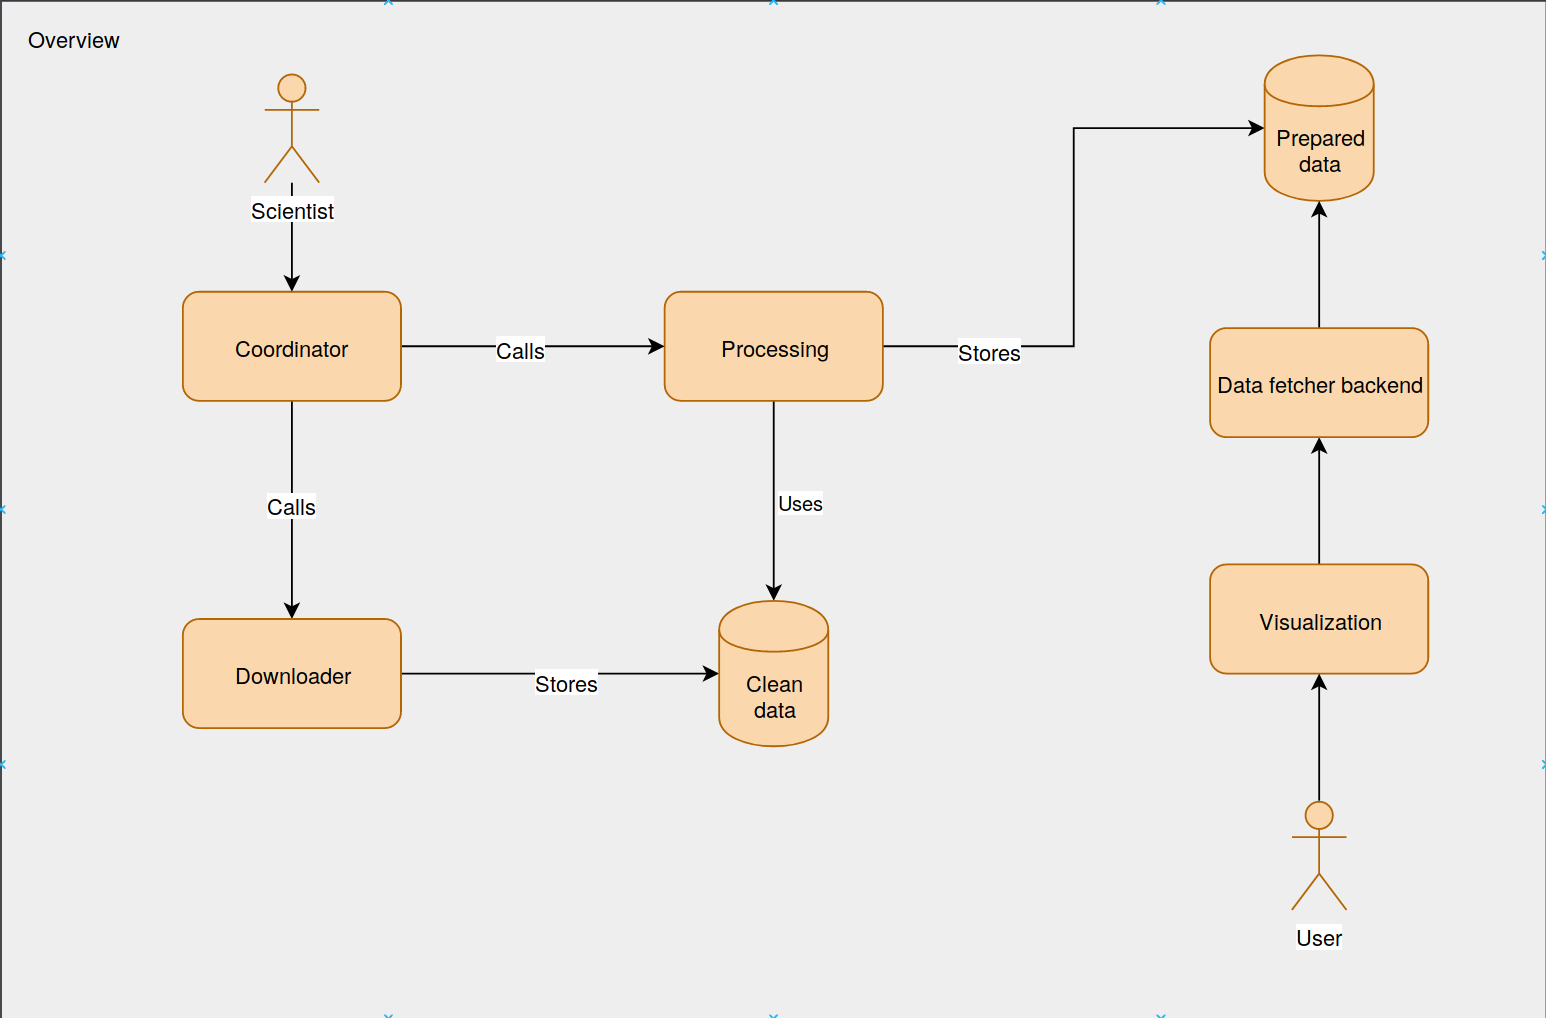
\includegraphics[width=10.5cm]{images/data_flow_overview.png}
	    	\caption{Data flow from database to \textit{k-means}}
	    	\label{fig:data_flow_pipeline}
  		\end{figure}
		
		    \vspace{1cm}
		    
	\clearpage
	
	\subsection{User interface}
	
	\subsubsection{User flow}
	
	\glspl{mockup} are created for desktop size application with \gls{drawio} diagramming tool.
	
	Happy path NEEDS CITATION is x and y, copy from scatter plot.
	
	. It can and be viewed in figures \ref{fig:frontend_mockup} and \ref{fig:frontend_mockup_2}. In figure \ref{fig:frontend_mockup} it is visible that  when user clicks landing page button, user is redirected to second screen with two tabs. Tab content can be visible together with filter controls. Clicking on tabs results into switching to another tab and can be seen on figure \ref{fig:frontend_mockup_2}.
	
	\begin{figure}[H]	
		\centering
		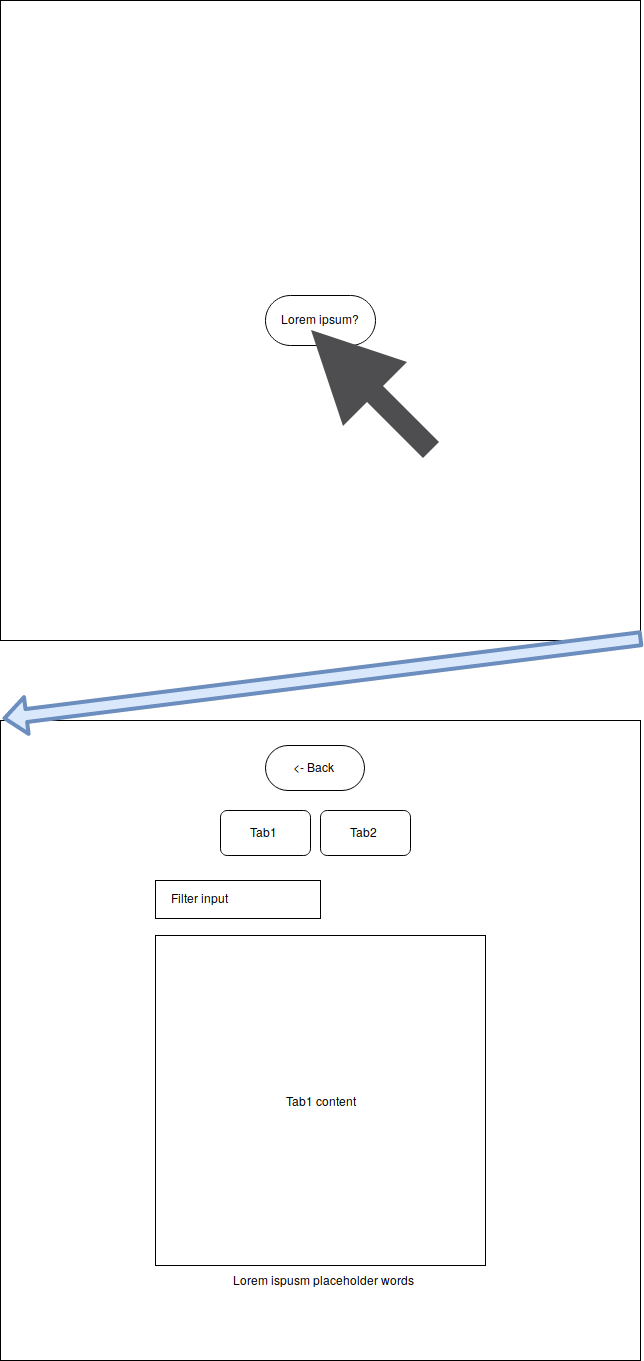
\includegraphics[width=9.5cm]{images/frontend_mockup_crop_1.png}
		\caption{Mockup of \gls{atviras_seimas} first screen}
		\label{fig:frontend_mockup}
	\end{figure}
	
	\begin{figure}[H]	
		\centering
		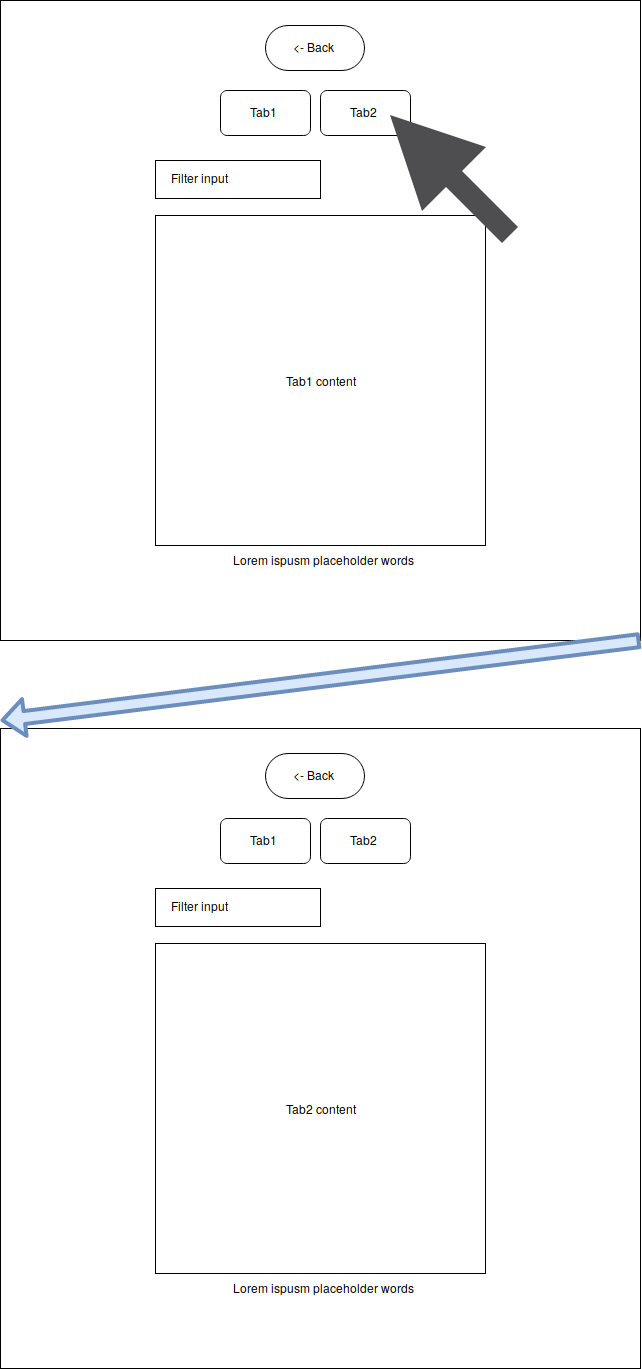
\includegraphics[width=9.5cm]{images/frontend_mockup_crop_2.png}
		\caption{Mockup of \gls{atviras_seimas} second screen}
		\label{fig:frontend_mockup_2}
	\end{figure}
	
	\subsubsection{Scatter plot}
	
	To visualize voting patterns data needs to be projected on two or one dimensional plot. Each dot represented can be different parliament member and its position can indicate its voting pattern. The more scattered two points are - the more different voting patterns are. Each point can have color of faction to easier indicate clusters with human eye. Another important feature is view different time periods, even arbitrarily chosen. This enables users to inspect differences during term of office.   
	Also it is worth to mention that parliament member change factions throughout term of office. For the sake of simplicity point color can be left to be faction color when member was elected to office. This approach has a drawback when looking at data changes during different periods, but it can keep things simplified.
	
	\subsubsection{Data filter}
	
	For users to inspect data with more than hundred points, filtering for members and factions needs to be present. Users are able to filter data by word. It is possible to filter by one word or phrase, however multiple words or phrases can also be used. In addition, while filtering data users can choose different periods of time. All this helps to compare separate factions to one another or parliament members to factions.
	
	\clearpage
	
	\begin{figure}[!tbp]
		\centering
		\subfloat[Data filter 1]{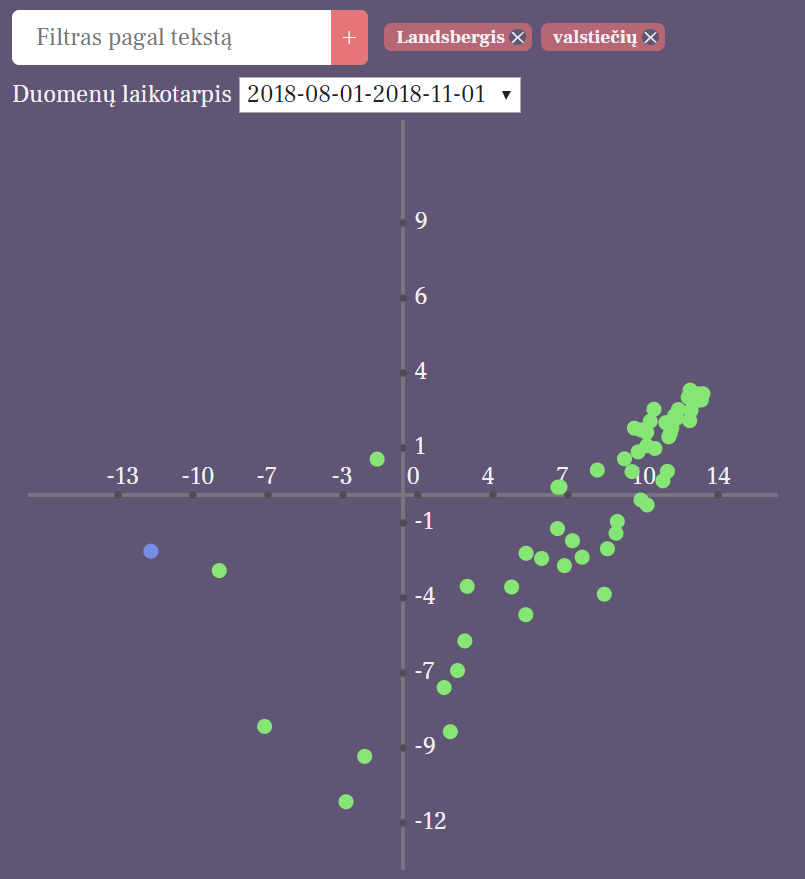
\includegraphics[width=0.4\textwidth]{images/filter1}\label{fig:f1}}
		\hfill
		\subfloat[Data filter 2]{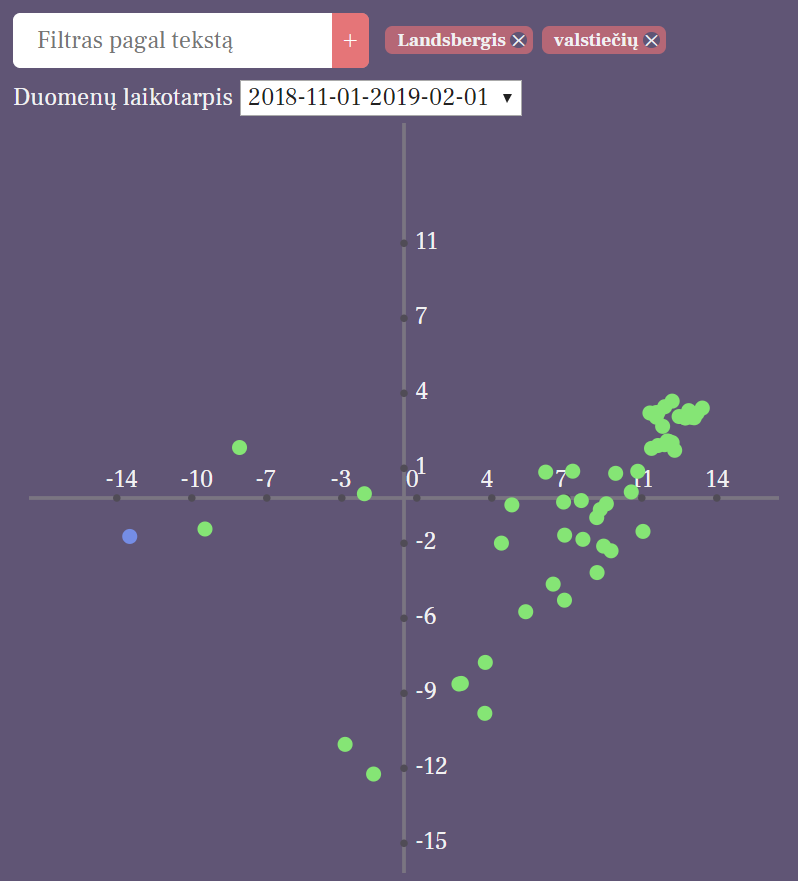
\includegraphics[width=0.4\textwidth]{images/filter2}\label{fig:f2}}
		\hfill
		\caption{Figure 4: Data filters}
	\end{figure}
	
	\clearpage

  	\subsection{Tools}
    \subsubsection{Programming language: {\textit Scala}}
    
    Both research and software parts of the project were done using \gls{scala} \cite{scala_lang}. \Gls{scala} choice is due its powerful type system and \gls{jvm} libraries accessibility \cite{scala_in_depth}. 
    
    \subsubsection{Database: {\textit MySQL}}
    
  	Since amount of data is relatively small as seen in experiment part - there is no need to consider data distribution problems. In this case the most important factor is to have fewer bugs. To achieve that \acrfull{sql} is picked which has types for each column - \gls{mysql} \cite{mysql_lang}.
    
	\subsection{API server}
	
	This subsystem handles incoming \gls{http} requests from users. It uses \textit{Akka-http} library \cite{akka_http}. Both computing and application requests are handled in this subsystem. Computing requests tell server to download specific set of data, update to newest data or order server to compute data for scientific methods. Application requests serve data to the client, querying it from the database. Since both client and server side are written with one programming language there are many benefits to use. While client side can remain as a single page application, server side can still share code with it. One such benefit - no need to write serializers and deserializers, since data types can be shared between two projects and process can be automatic. 
	
	\subsection{Coordinator}
        
    \subsection{Downloader}
    
    Downloader consists of few parts: \textit{Download coordinator, Scraper, Parser, Error handler}. 
    
 
%    \subsection{Repository}
    \clearpage
    
    \section{Description of experimental research}
    \subsection{Data statistics}
    
   	Data statistics are calculated from data \gls{lrs_open} \acrshort{api} which was downloaded and saved to local database. Quite a big chunk data from 1990-2012 is missing due different information systems used at that time and other reasons. It was not migrated to current open data \acrshort{api}. For this reason this project focuses more on recent data, but it is not limited to analyze older data too if it becomes available.
    
   	\noindent
    \begin{center}
    	\begin{tabular}{L{5cm} R{3cm}}
    		\multicolumn{2}{c}{}\\ 
    		\hline
    		Name & Count \\\hline
    		Terms of office & 8\\
    		Sessions & 101\\
    		Parliament members & 1207\\
    		Plenaries & 3977\\
    		Vote rows & 3933006\\
    		Votes & 28121\\
    		Agenda questions & 64243\\
    		Plenary questions (2012-) & 15108\\
    		Discussion events (2007-) & 361996\\
    		\hline
    	\end{tabular}
    	\captionof{table}{Statistics of downloaded data} \label{tab:data_statistics}
    \end{center}

    
    \hfill 
    
   	\subsection{Encoding of data} 
   	
   	To use scientific methods data needs to be prepared for them. Two methods: \textit{\acrshort{mds}} and \gls{k-means} need distances between pairs or training rows to compare parliament members to each other. This means that to compare one member's to another some measure like \gls{euclidian} is needed to produce numerical difference between points. Vote outcomes in given data are categorical, meaning they need to be converted to numbers. Since authors in  \cite{vytautas_mick_magistrinis} tried few vote encoding for \acrshort{mds} and \gls{lrs} older data - this project will use different ones to capture broader scientific results. Data for experiments only includes current term, which start in 2016.
   	
   	In table \ref{tab:vote_outcome_encoding} chosen voting outcomes encoding can be viewed. \textit{Encoding 1} straightforward scores are chosen. Voting abstain has negative score, because some legislature requires absolute majority to pass, therefore minority of parliament can block by abstaining. Did not vote is considered to be neutral, as some parliament members begin their term of office later and need to be assigned a score. \textit{Encoding 2} values are chosen more flexibly. Voting for and against are opposites, however voting abstain and not attending are neutral. This is to cover the case where members actually vote not to block specific vote, but don't have opinion on what to vote. \textit{Encoding 3} differs by having negative score for not voting at all. This is to cover the case where half or parliament members plus one is needed to pass certain laws, like changing constitution. This means that by not registering to vote you can actually vote against \cite{konstitucija}.
 
 	\noindent
   	\begin{center}
   		\begin{tabular}{L{3cm} C{2cm} C{2cm} C{2cm}}
   			\multicolumn{2}{c}{}\\ 
   			\hline
   			Vote outcome & Encoding 1 & Encoding 2& Encoding 3  \\\hline
   			For & 2 & 1 & 2 \\
 			Against & -2 & -1 & -2\\
 			Abstain & -1 & 0 & -1\\
 			Did not vote & 0 & 0 & -1\\
   			\hline
   		\end{tabular}
   		\captionof{table}{ Encoding of vote outcomes} \label{tab:vote_outcome_encoding}
   	\end{center}
   
   	Since factions are important part when viewing visualizations, they need to be consistent throughout graphs. Faction assigned colors can be viewed in figure 
   	
 	\begin{figure}[H]	
  		\centering
  		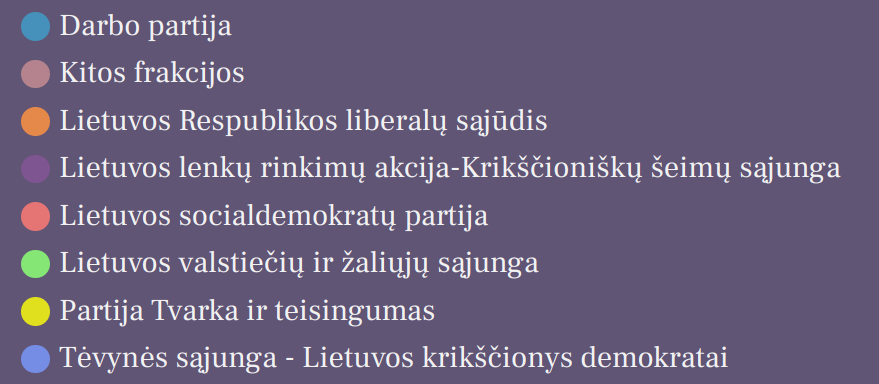
\includegraphics[width=9.5cm]{images/faction_colors.png}
  		\caption{Colors assigned to factions in following visualizations}
  		\label{fig:faction_colors}
   	\end{figure}
   
   	\clearpage
   	   	
   	\subsection{Multidimensional Scaling}
   	
   	To use \acrshort{mds} method proximity matrix needs to be generated. Distances need to be calculated from given data. Goal is to view voting patterns for given parliament members meaning that connection between somehow encoded votes and parliament members needs to be represented with this matrix.
   	
   	In figures \ref{fig:mds_e1}, \ref{fig:mds_e2}, \ref{fig:mds_e3} MDS for current term of office is calculated and projected on 2d scatter plot. Three variants show how different vote encoding changes plot. Table \ref{tab:mds_performance]} shows that \textit{E2 encoding} has the highest proportion of variance of the scaled data which was accounted by MDS method. It shows that \textit{E2 encoding} loses the least amount of data, meaning simple vote for and vote against is the best encoding for this case. Also, in visualization, faction voting patterns are clearly visible, as member votes are close to each other. Forming clusters.
   	
   	\noindent
   	\begin{center}
   		\begin{tabular}{L{2cm} C{4cm}}
   			\multicolumn{2}{c}{}\\ 
   			\hline
   			Encoding & Proportion of variance \\\hline
   			E1 & 0.752 \\
   			E2 & 0.790 \\
   			E3 & 0.764 \\
   			\hline
   		\end{tabular}
   		\captionof{table}{ Proportion of variance for MDS} \label{tab:mds_performance]}
   	\end{center} 
   
   	\begin{figure}[!tbp]
   	\centering
   	\subfloat[encoding = E1]{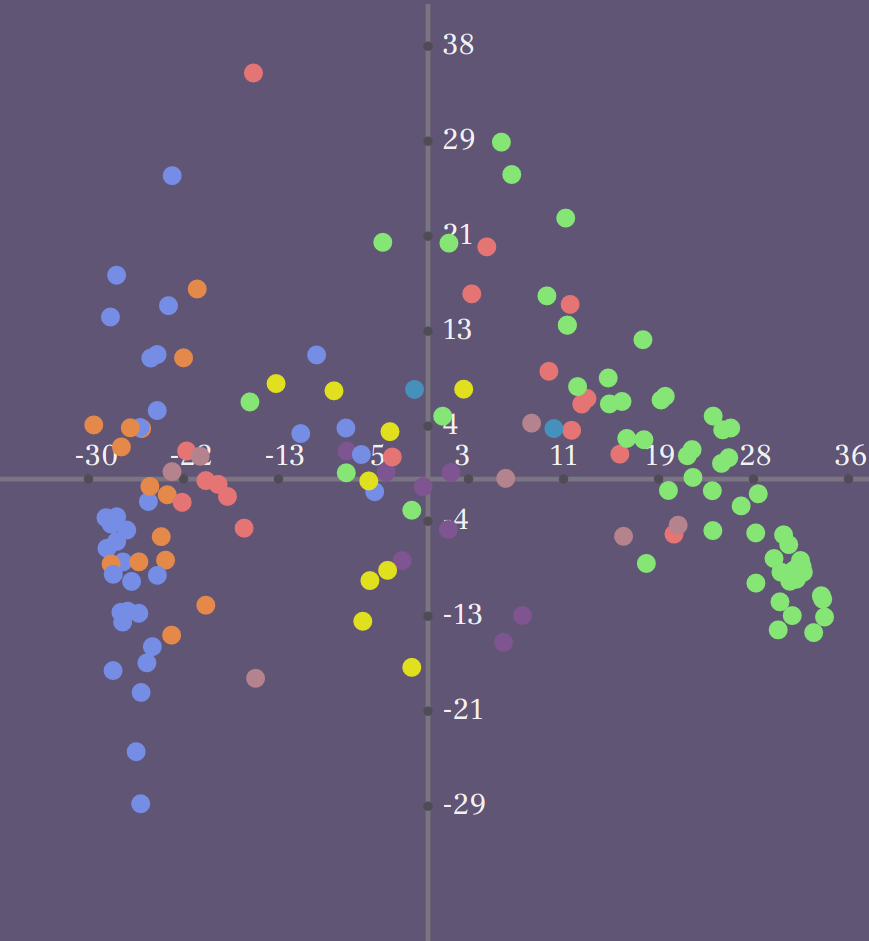
\includegraphics[width=0.48\textwidth]{images/mds_e1}\label{fig:mds_e1}}
   	\hfill
   	\subfloat[encoding = E2]{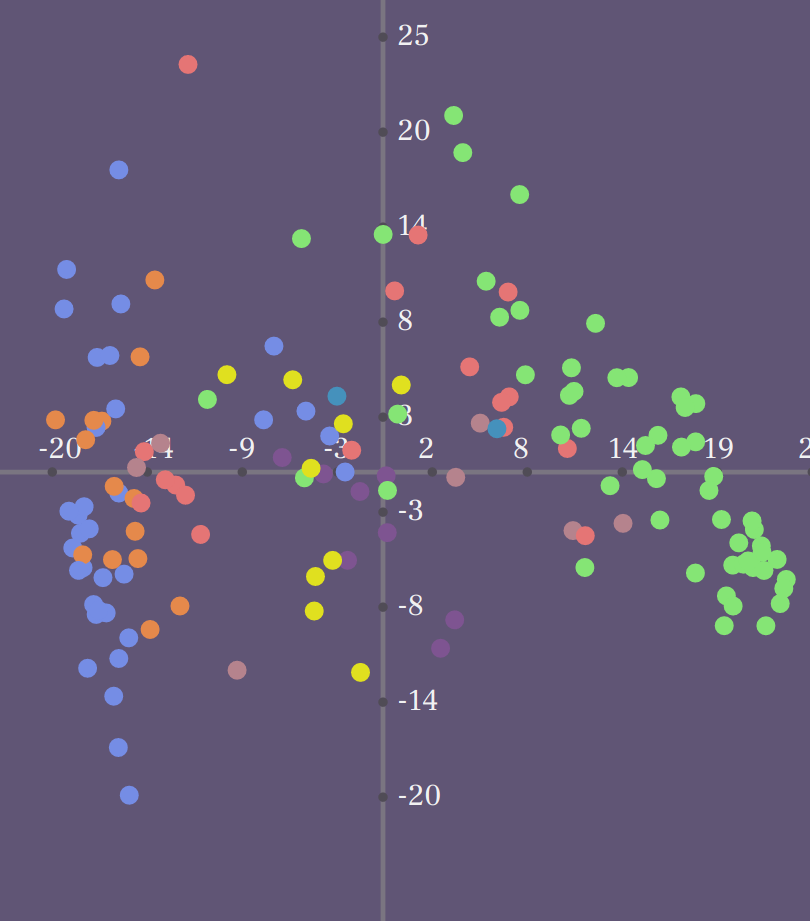
\includegraphics[width=0.46\textwidth]{images/mds_e2}\label{fig:mds_e2}}
   	\hfill
   	\subfloat[encoding = E3]{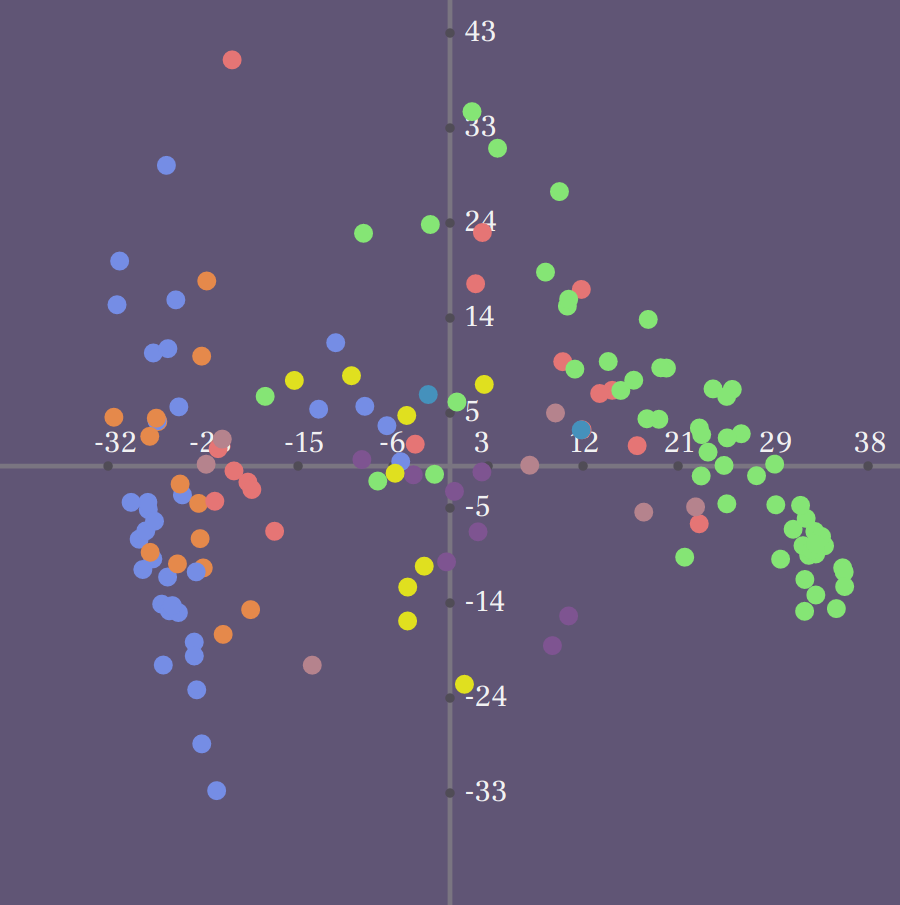
\includegraphics[width=0.46\textwidth]{images/mds_e3}\label{fig:mds_e3}}
   	\caption{MDS on 2d scatter plot}
   \end{figure}
  	   	
   	\clearpage
   	
   \subsubsection{Time periods}
   	
   	To get more insights, as discussed in problem analysis, data is split into 91.25 day periods. This enables to see what difference each of these periods introduce to the members. For example: Justas Džiugelis was a member of Greens majority faction during 2016-11-14 – 2018-09-10 period. If \gls{mds} were plotted to show how his voting is similar to his faction during current term of office - its possible to see how farther he gets before leaving the party. Comparison can be seen in figure \ref{fig:justas_all}, where green dots are members from his former faction, and light blue point is him. Before he leave the party on 2018-09-10, his voting patterns start to diverge starting 2018-02-01 voting period.
   	
   	 	\begin{figure}[!tbp]
   		\centering
   		\subfloat[2016-11-01 --- 2017-02-01]{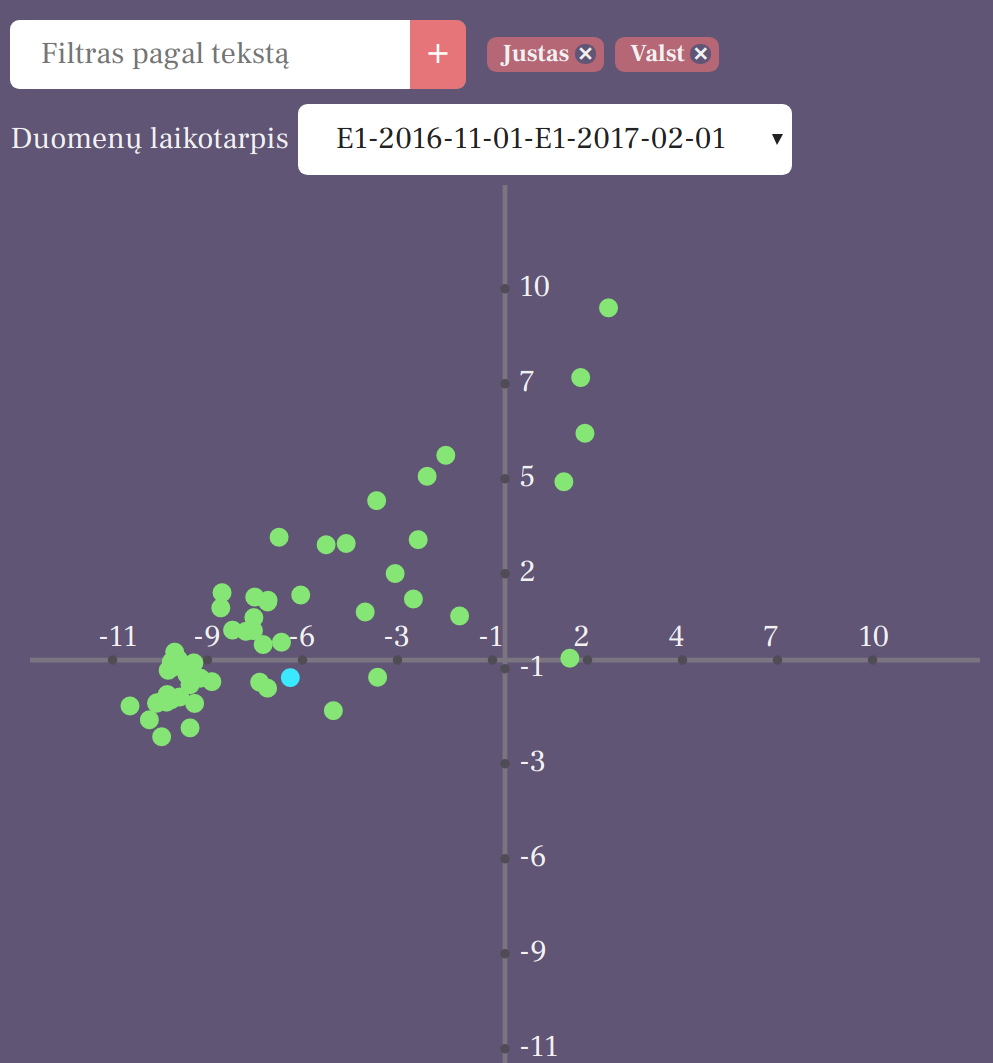
\includegraphics[width=0.31\textwidth]{images/justas1}\label{fig:justas1}}
   		\hfill
   		\subfloat[2017-02-01 --- 2017-05-01]{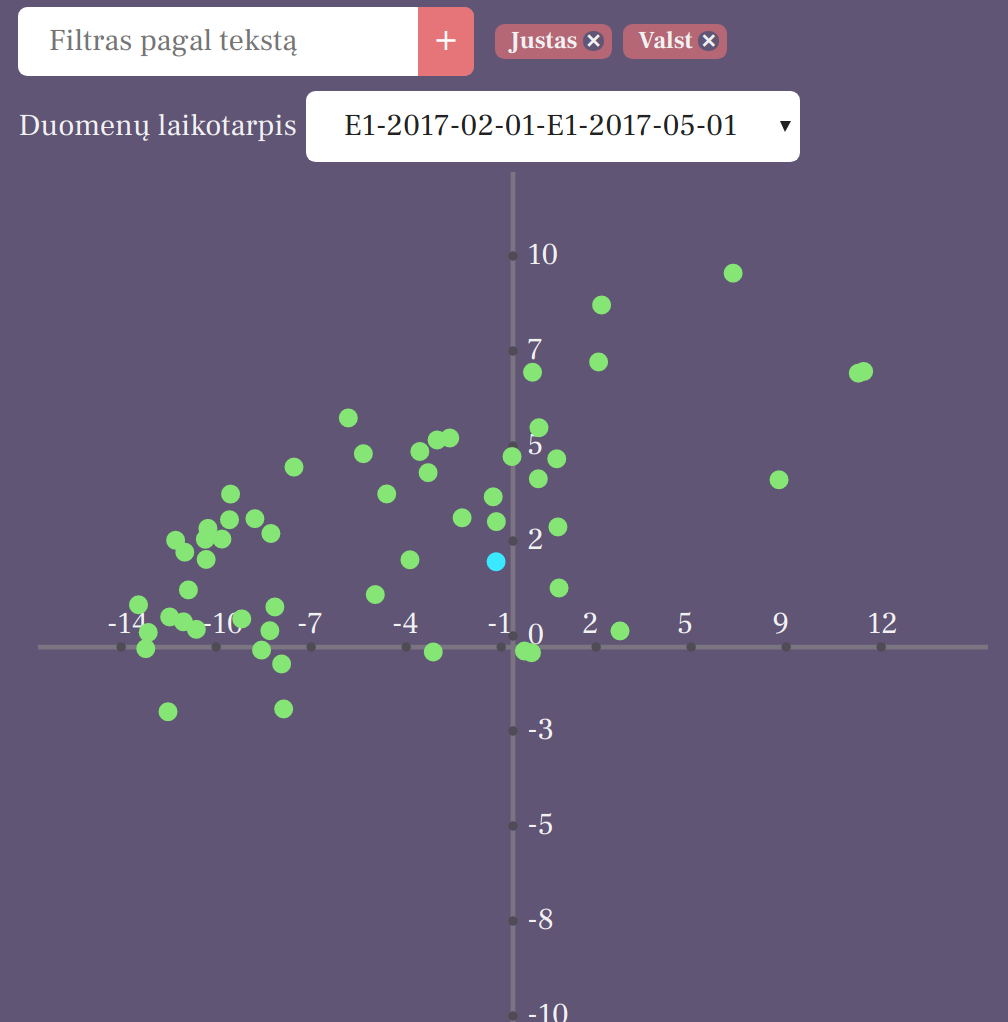
\includegraphics[width=0.31\textwidth]{images/justas2}\label{fig:justas2}}
   		\hfill
		\subfloat[2017-05-01 --- 2017-08-01]{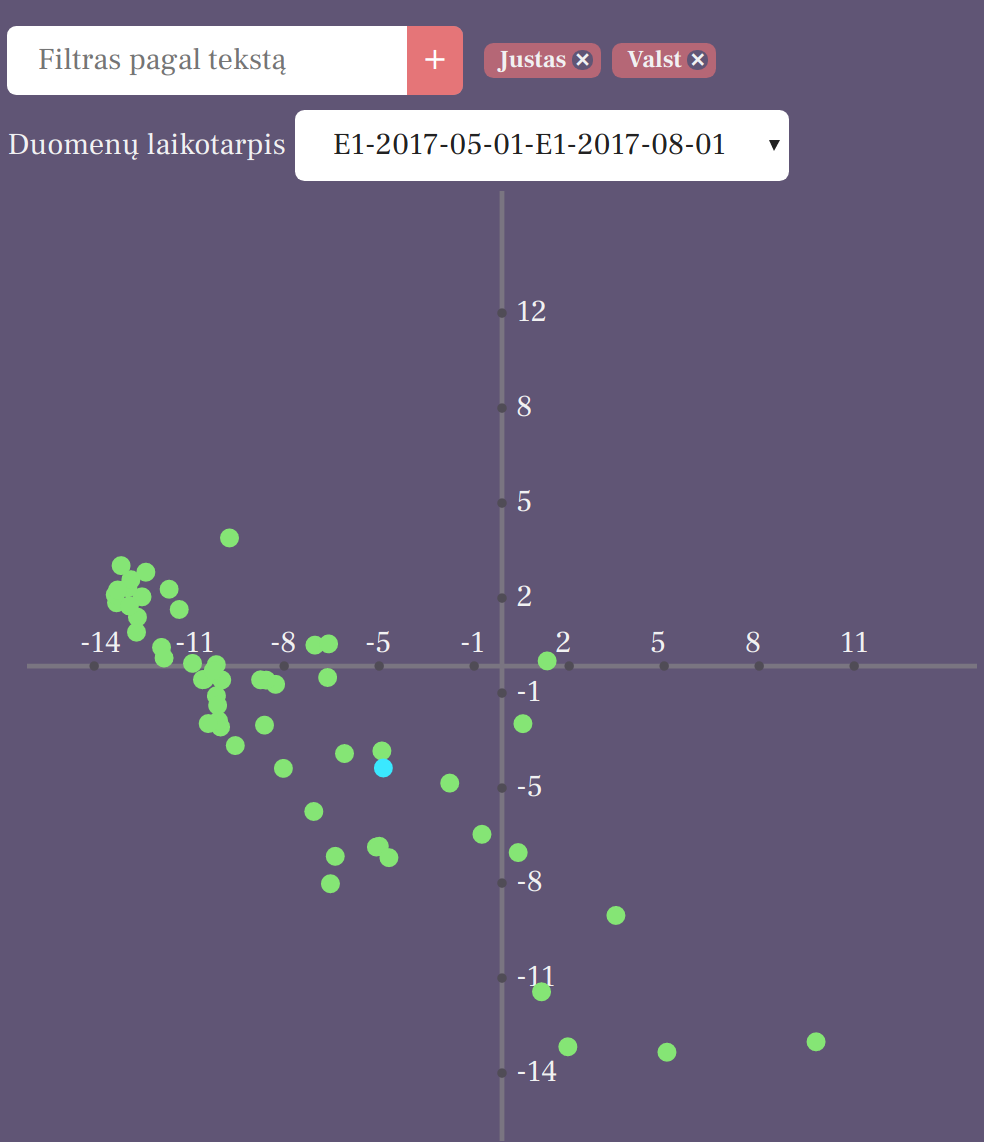
\includegraphics[width=0.31\textwidth]{images/justas11}\label{fig:justas11}}
   		\hfill
   		\subfloat[2017-08-01 --- 2017-11-01]{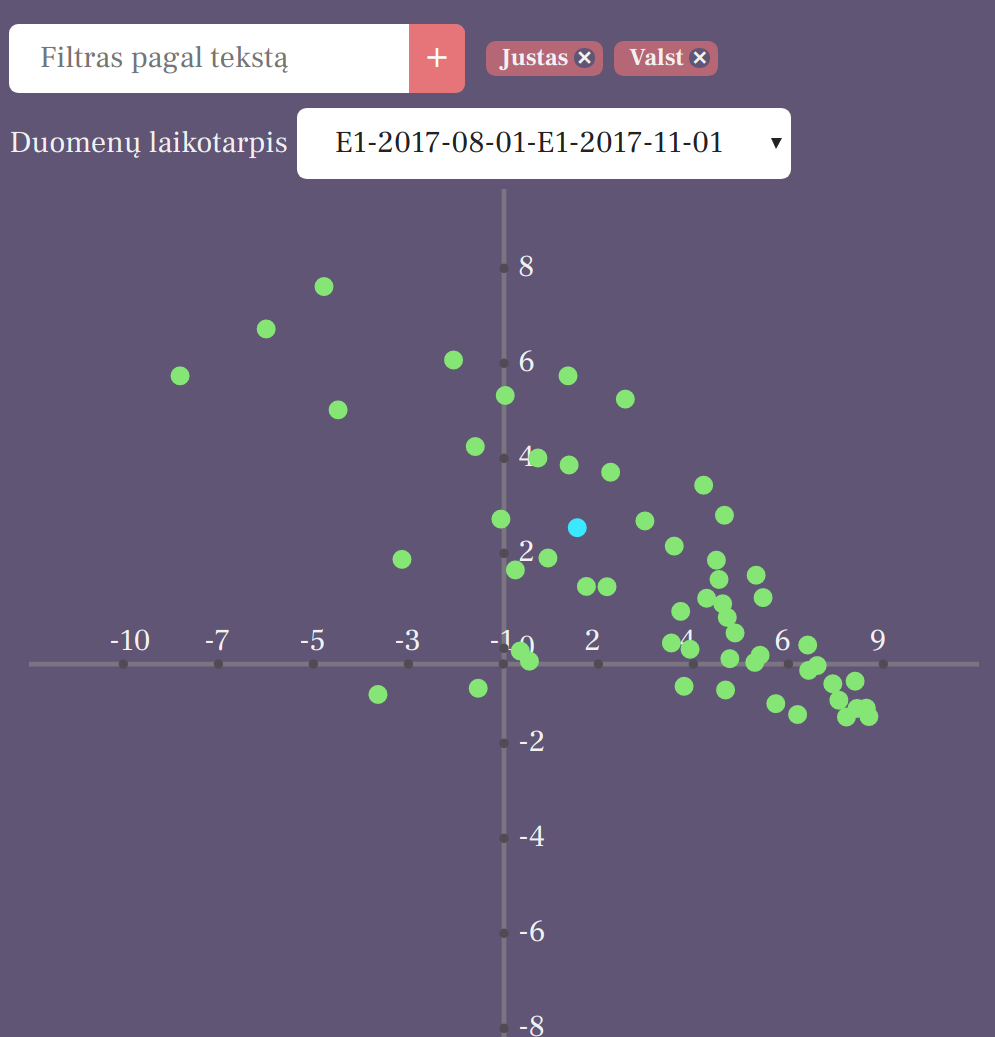
\includegraphics[width=0.31\textwidth]{images/justas4}\label{fig:justas4}}
   		\hfill
   		\subfloat[2017-11-01 --- 2018-02-01]{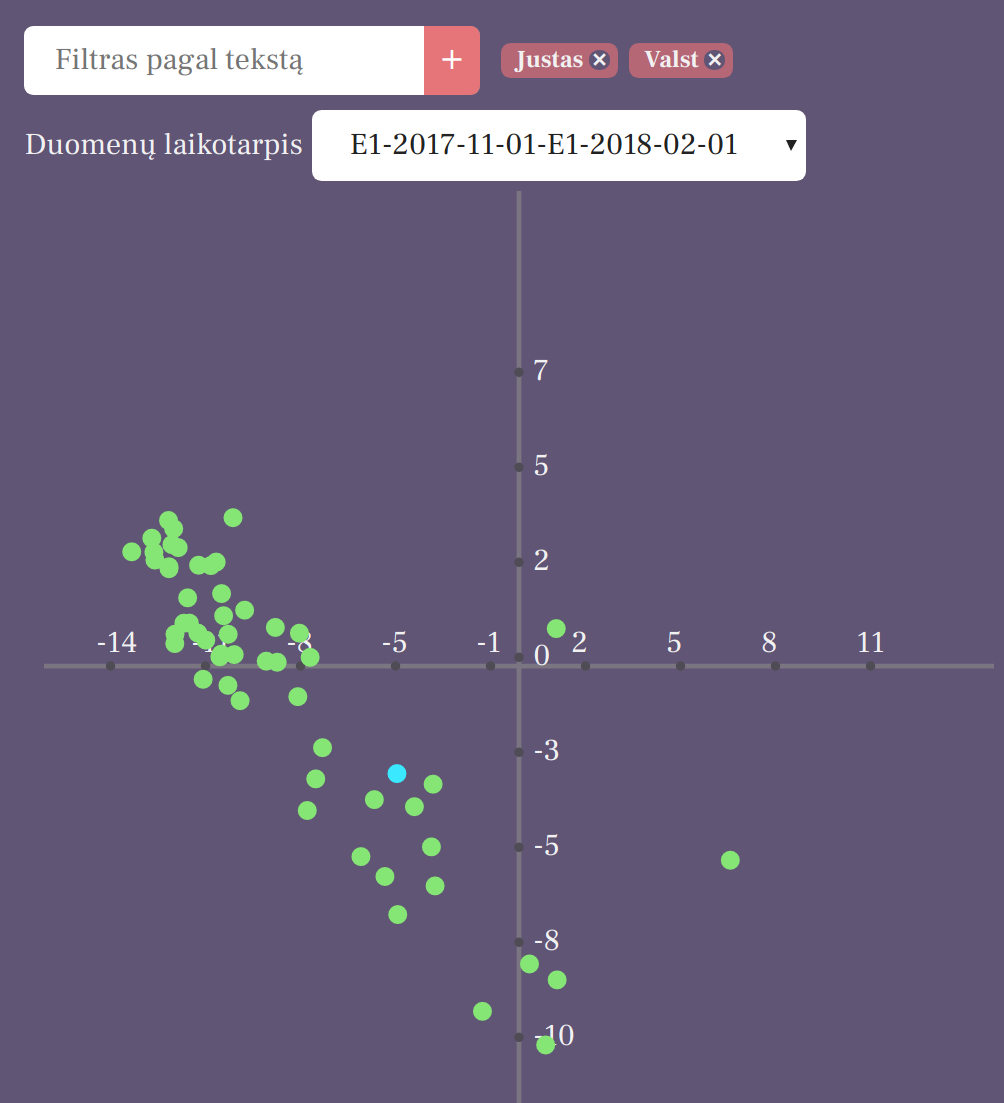
\includegraphics[width=0.31\textwidth]{images/justas5}\label{fig:justas5}}
   		\hfill
		\subfloat[2018-02-01 --- 2018-05-01]{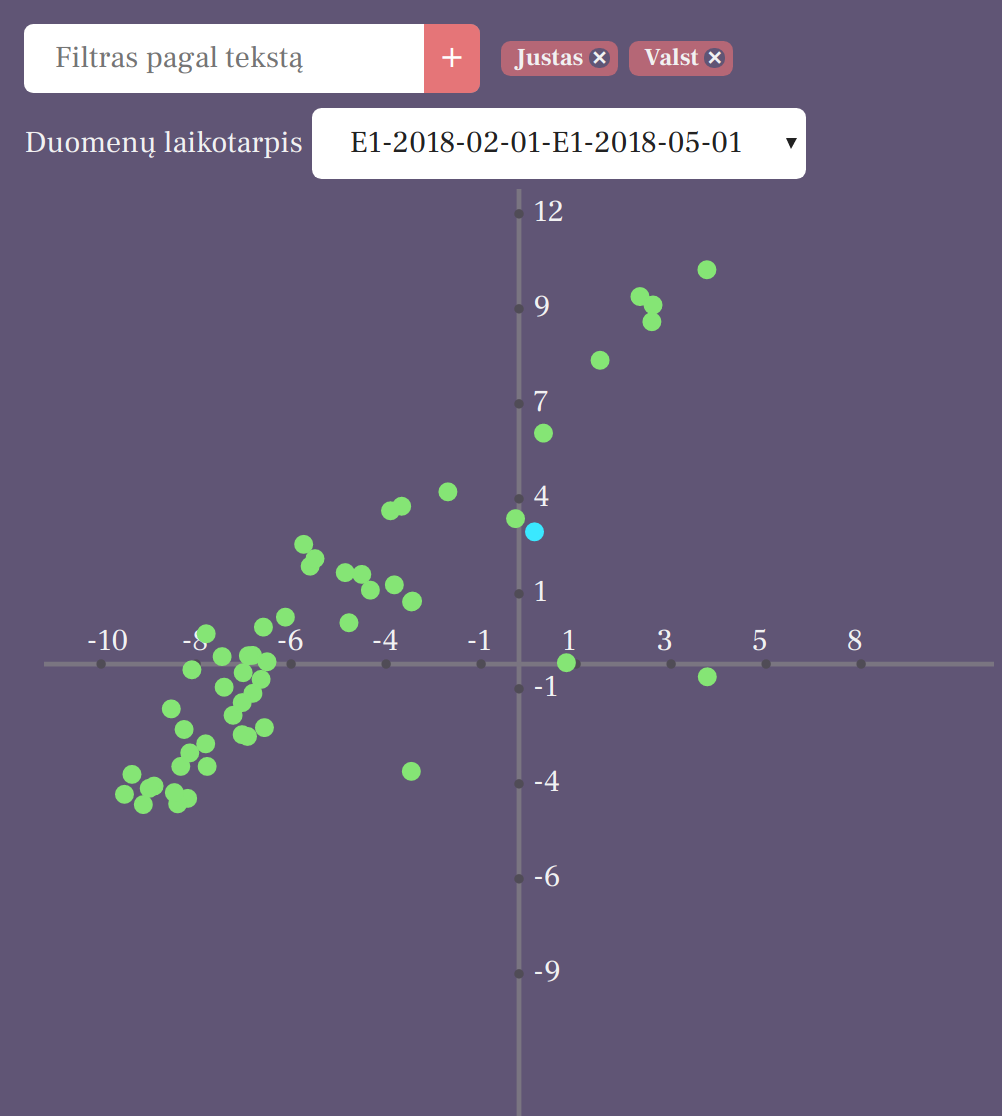
\includegraphics[width=0.31\textwidth]{images/justas6}\label{fig:justas6}}
		\hfill
		\subfloat[2018-05-01 --- 2018-08-01]{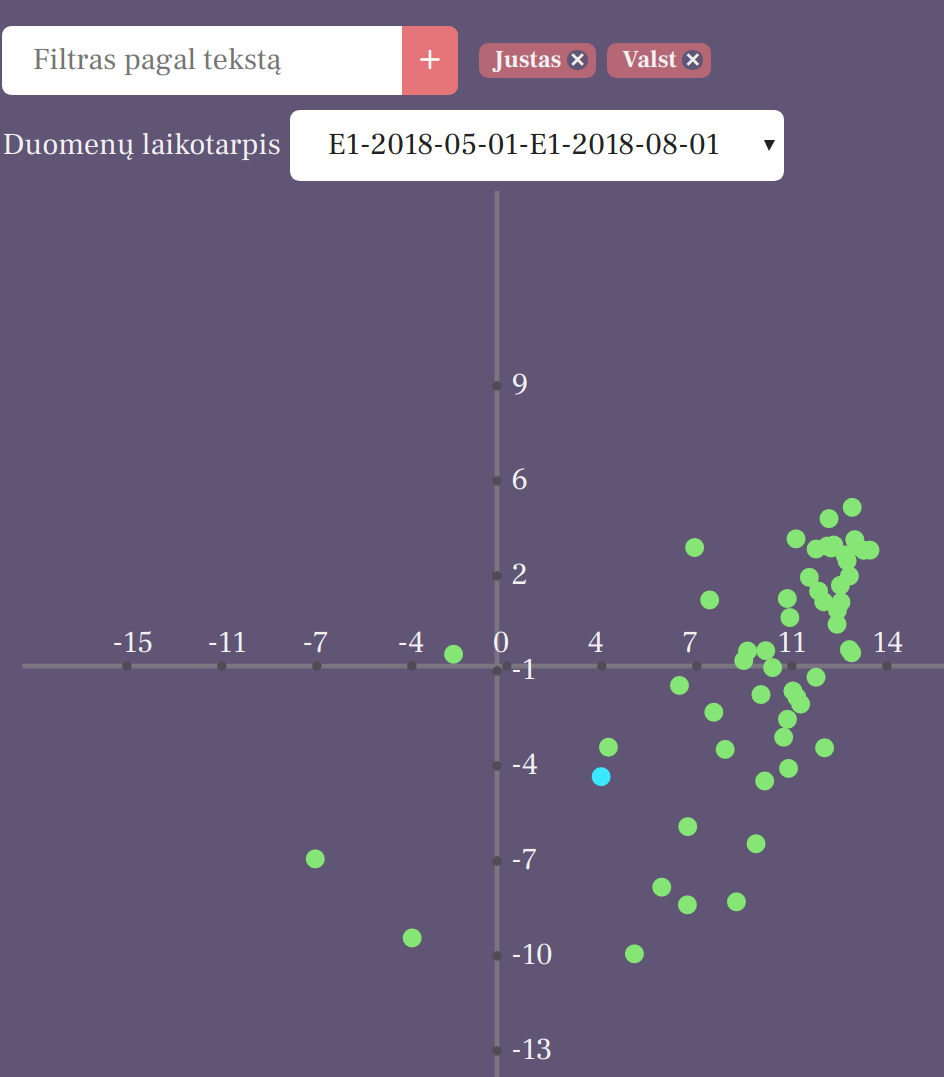
\includegraphics[width=0.31\textwidth]{images/justas7}\label{fig:justas7}}
		\hfill
		\subfloat[2018-08-01 --- 2018-11-01]{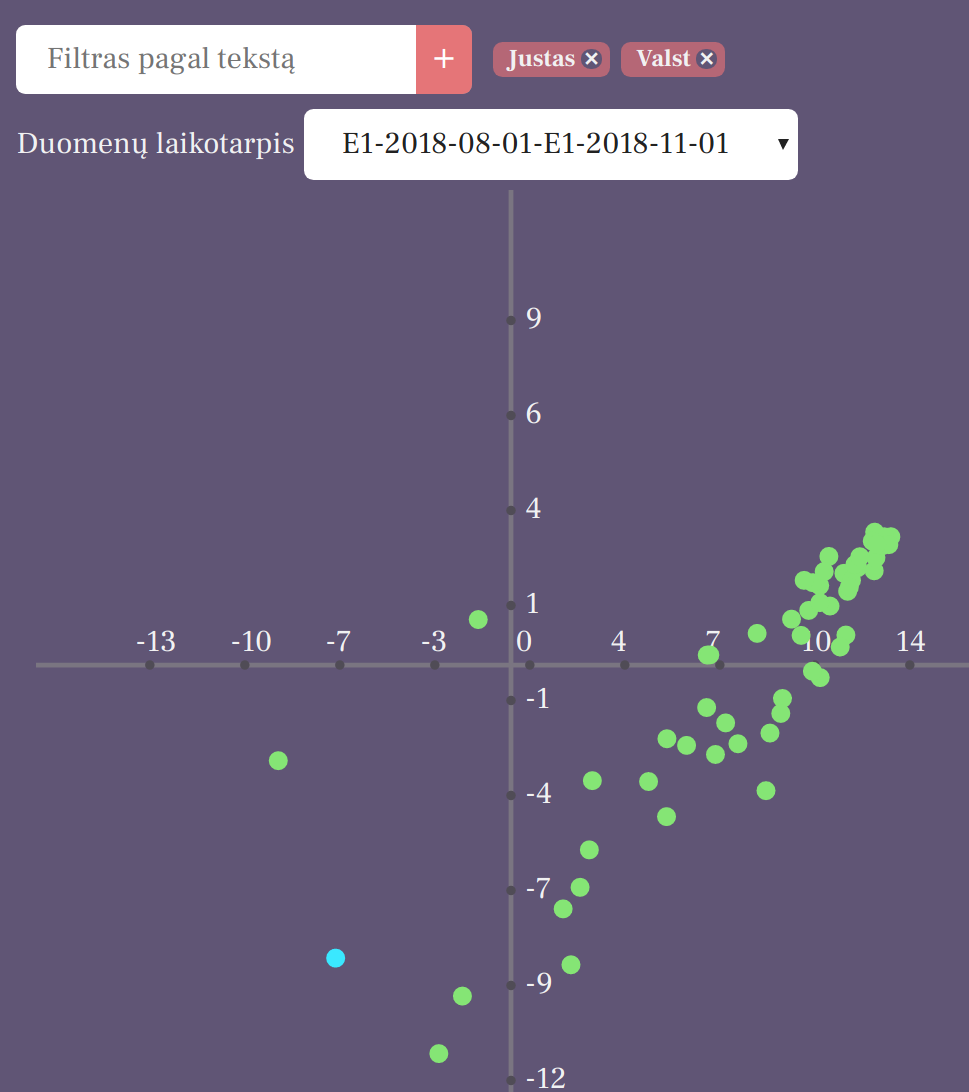
\includegraphics[width=0.31\textwidth]{images/justas8}\label{fig:justas8}}
		\hfill
		\subfloat[2018-11-01 --- 2019-02-01]{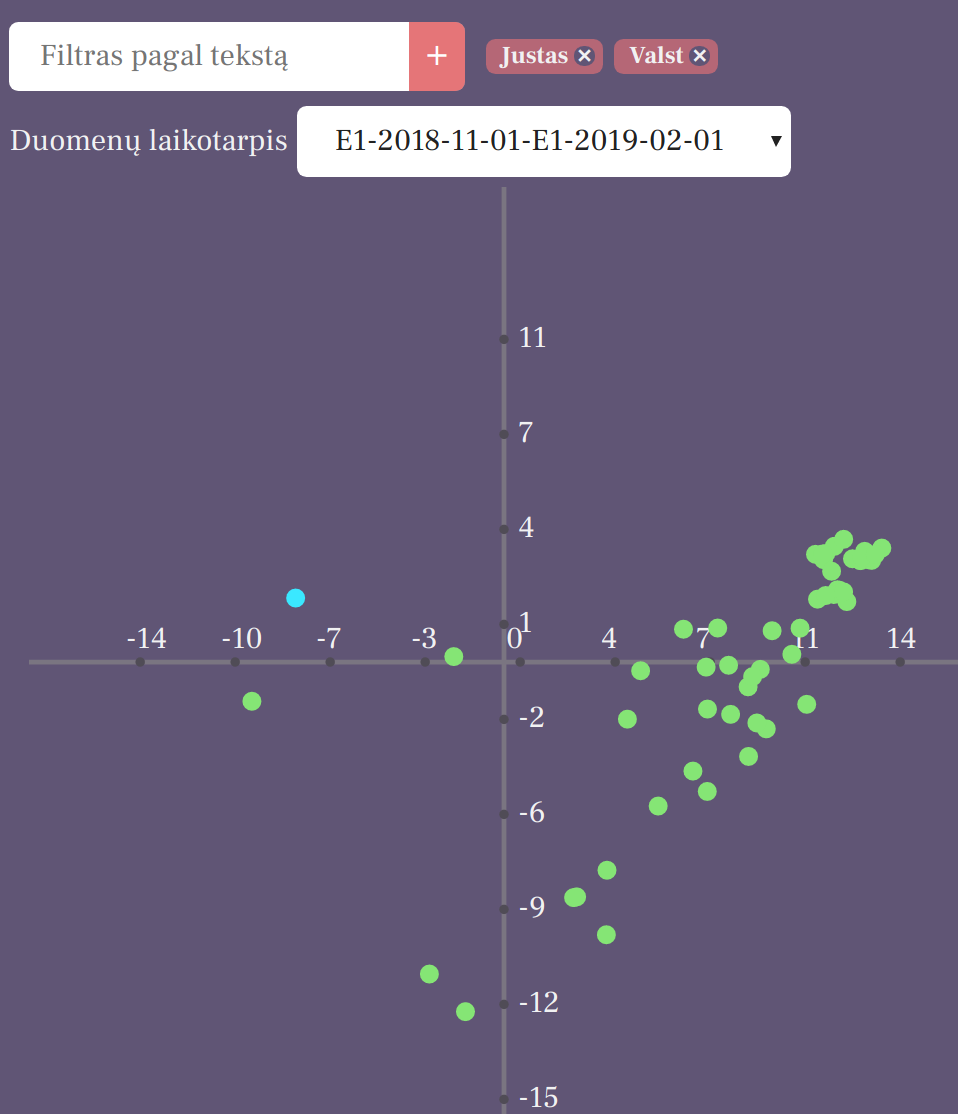
\includegraphics[width=0.31\textwidth]{images/justas9}\label{fig:justas9}}
		\hfill	
   		\caption{Changes in Justas Džiugelis voting patterns}
   		\label{fig:justas_all}
   	\end{figure}
   
   \clearpage
   	
   	\subsection{Unsupervised learning: {\textit k-means} clusterization }
   	
   		
   	There are two goals for \gls{k-means}: classify majority from minority and see if there are groups not explicitly split into factions.
   	
   	Since some members joined parliament after term of office start or left it before it ended - data is missing on their votes during that time. To avoid this issue - empty training rows are added for that missing time.
   	
	Results from \gls{k-means} are displayed on \acrshort{mds} calculated coordinates for the same time period. Training rows for clustering are prepared by encoding votes for given parliament member. Iteration count is 20.
	
	\subsubsection{Majority vs minority} 
	
	Majority and minority are two groups which usually have different ideologies - they couldn't group up, therefore are voting differently on issues. Another experiment could be to test three groups - two for minority and majority and one for outsides, parliament members who left one group or another, changed parties or are voting individually.
	
	Figures \ref{fig:majority_vs_minority_k2_e1}, \ref{fig:majority_vs_minority_k2_e2}, \ref{fig:majority_vs_minority_k2_e3} can be observed for results projected on MDS coordinates with fixed encoding \textit{E1} for the same time period. Graphs show how parliament members are assigned to two clusters. Just from visual part it is not clear which encoding has best performance. From \Gls{k-means} \textit{distortion} in table \ref{tab:k_means_performance} shows \textit{E2 encoding} to have the lowest value. Closer look at \ref{fig:majority_vs_minority_k2_e2} suggests that most of points are classified correctly in this graph, white points being a minority and blue ones belonging to majority. This finding can also suggest that simple vote for and vote against split for positive negative score is the best as it was for MDS proportion of variance.
	
	
	\noindent
	\begin{center}
		\begin{tabular}{L{3cm} C{2cm} C{2cm} C{2cm}}
			\multicolumn{2}{c}{}\\ 
			\hline
			Encoding & k=2 & k=3 \\\hline
			E1 & 536738 & 500433 \\
			E2 & 121566 & 116326 \\
			E3 & 854237 & 811270 \\
			\hline
		\end{tabular}
		\captionof{table}{ Distortion for \gls{k-means} majority vs minority results} \label{tab:k_means_performance}
	\end{center} 
	
	\begin{figure}[!tbp]
		\centering
		\subfloat[k=2, encoding = E1]{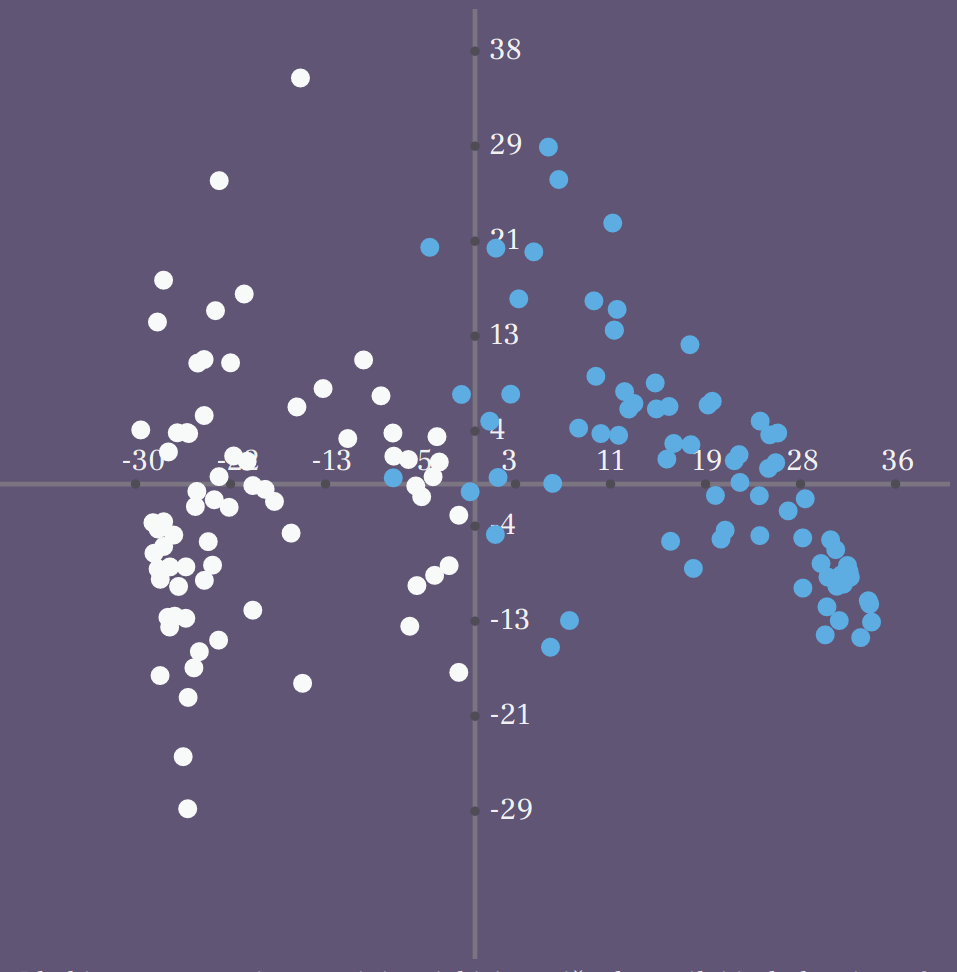
\includegraphics[width=0.46\textwidth]{images/kmeans_k2_e1}\label{fig:majority_vs_minority_k2_e1}}
		\hfill
		\subfloat[k=2, encoding = E2]{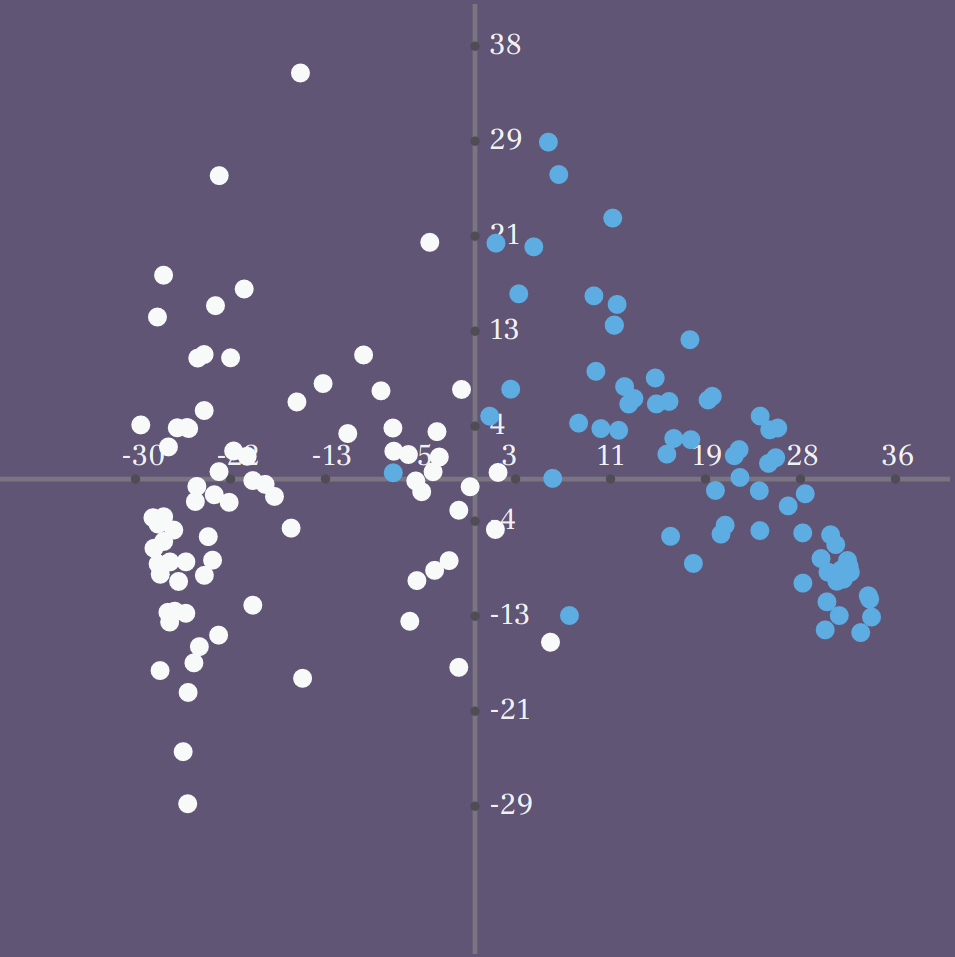
\includegraphics[width=0.46\textwidth]{images/kmeans_k2_e2}\label{fig:majority_vs_minority_k2_e2}}
		\hfill
		\subfloat[k=2, encoding = E3]{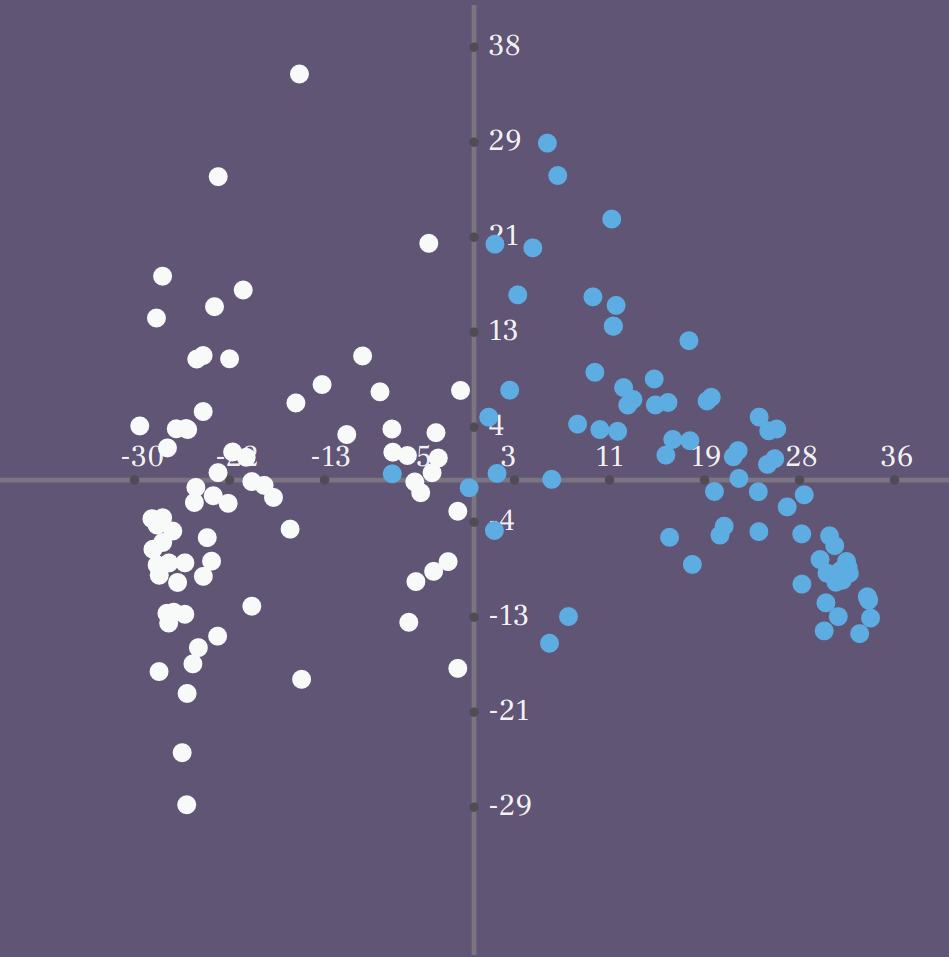
\includegraphics[width=0.46\textwidth]{images/kmeans_k2_e3}\label{fig:majority_vs_minority_k2_e3}}
		\caption{majority vs minority, \gls{k-means} on \acrshort{mds} coordinates}
	\end{figure}
	
	\clearpage

	Looking at figures \ref{fig:majority_vs_minority_k3_e1},\ref{fig:majority_vs_minority_k3_e2}, \ref{fig:majority_vs_minority_k3_e3} suggests that \textit{k=3} is one cluster too much for \textit{E2, E3} encodings as it doesn't show anything meaningful. \ref{fig:majority_vs_minority_k3_e1} figure looks more shows points which are more truthful, white points being people who are outsiders as predicted in hypothesis. 

	\begin{figure}[!tbp]
	\centering
	\subfloat[k=3, encoding = E1]{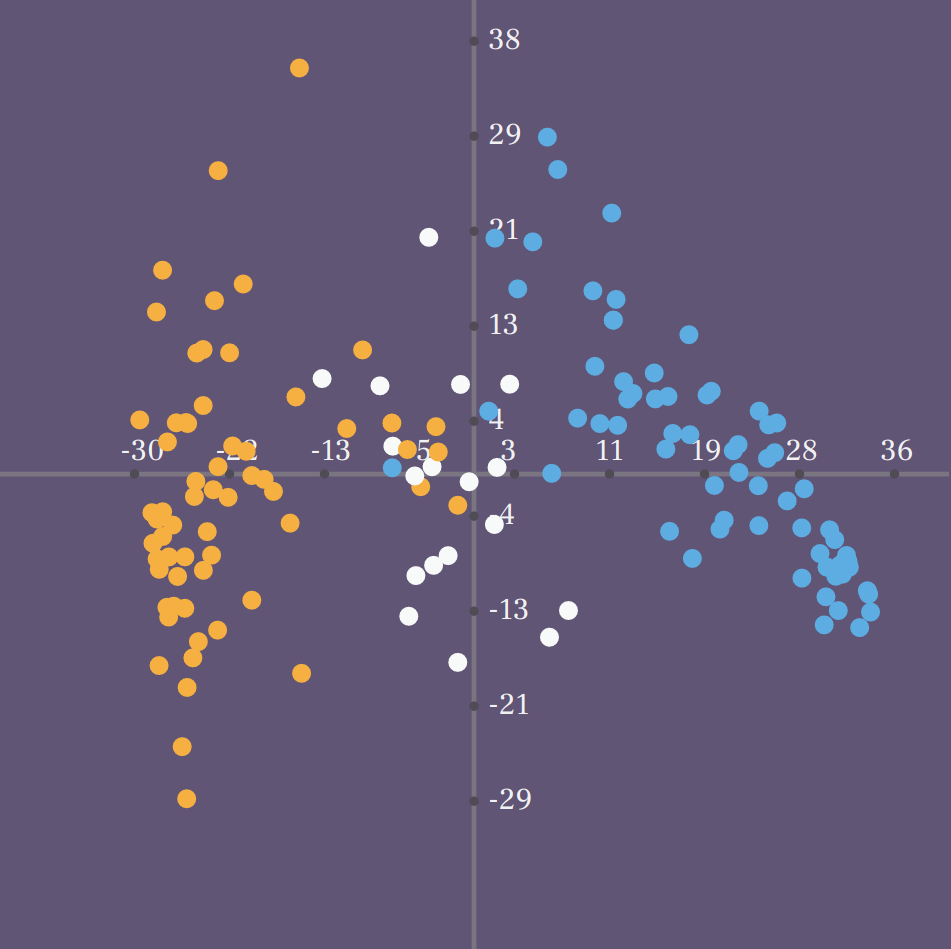
\includegraphics[width=0.46\textwidth]{images/kmeans_k3_e1}\label{fig:majority_vs_minority_k3_e1}}
	\hfill
	\subfloat[k=3, encoding = E2]{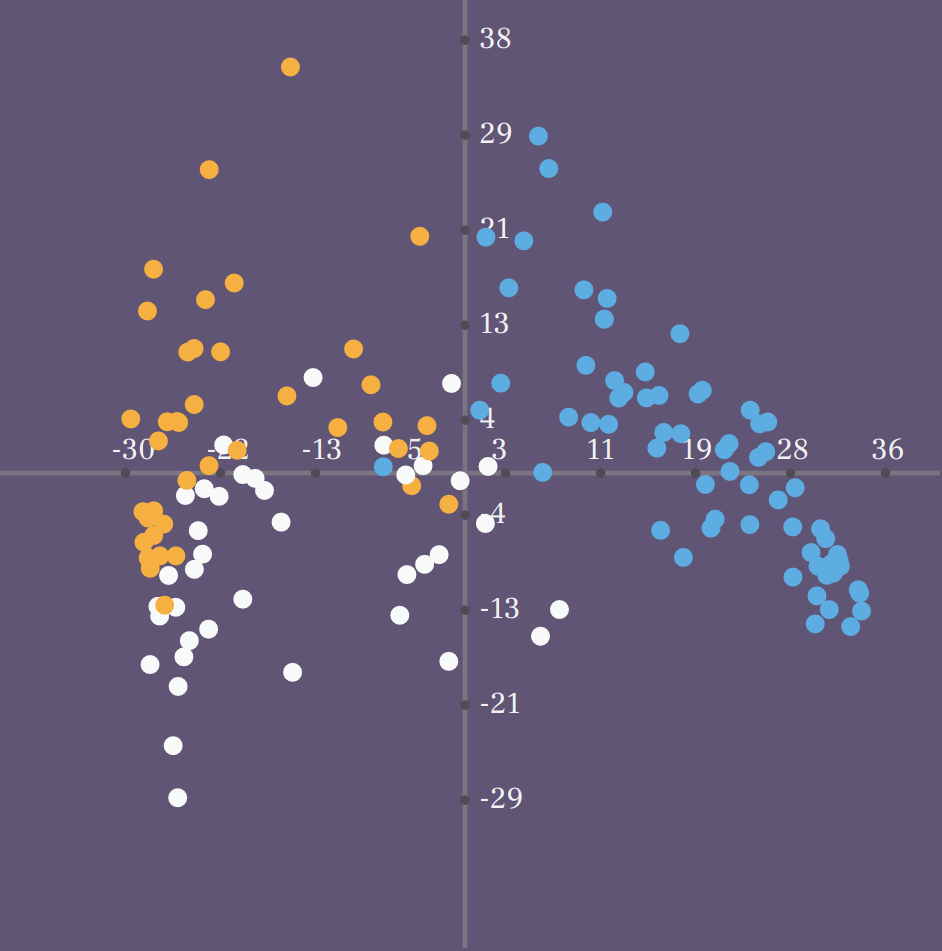
\includegraphics[width=0.46\textwidth]{images/kmeans_k3_e2}\label{fig:majority_vs_minority_k3_e2}}
	\hfill
	\subfloat[k=3, encoding = E3]{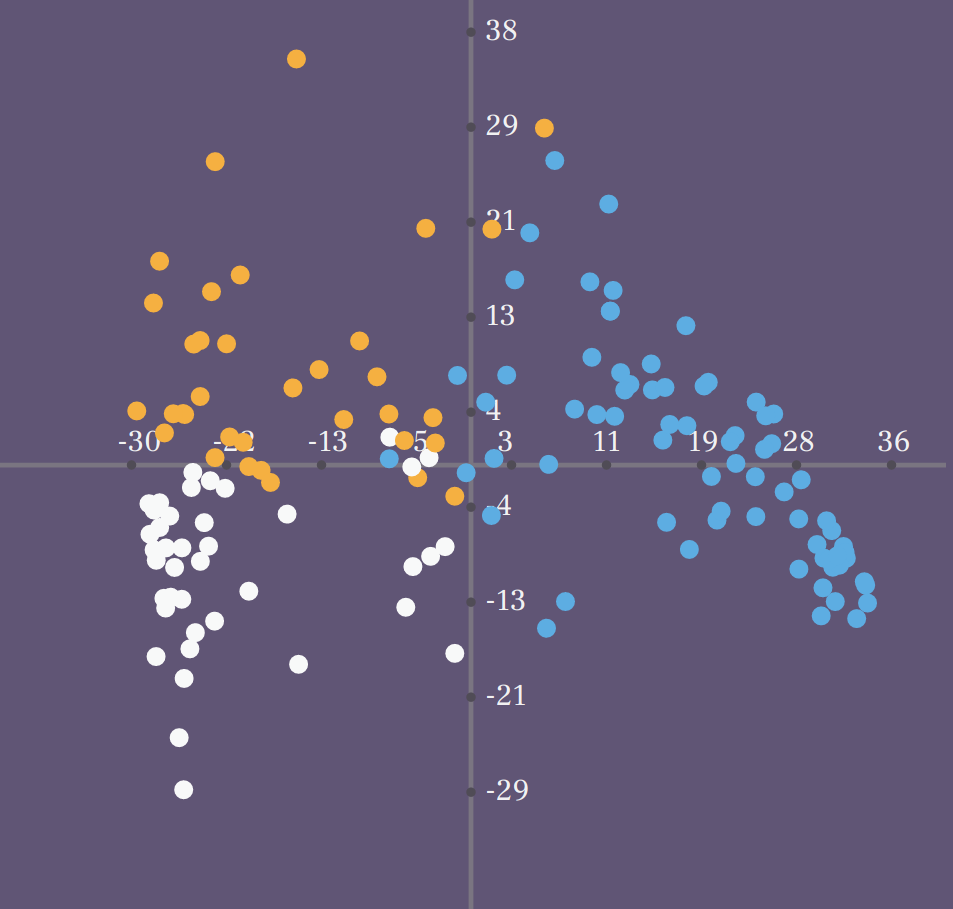
\includegraphics[width=0.46\textwidth]{images/kmeans_k3_e3}\label{fig:majority_vs_minority_k3_e3}}
   	\hfill
	\subfloat[Actual factions]{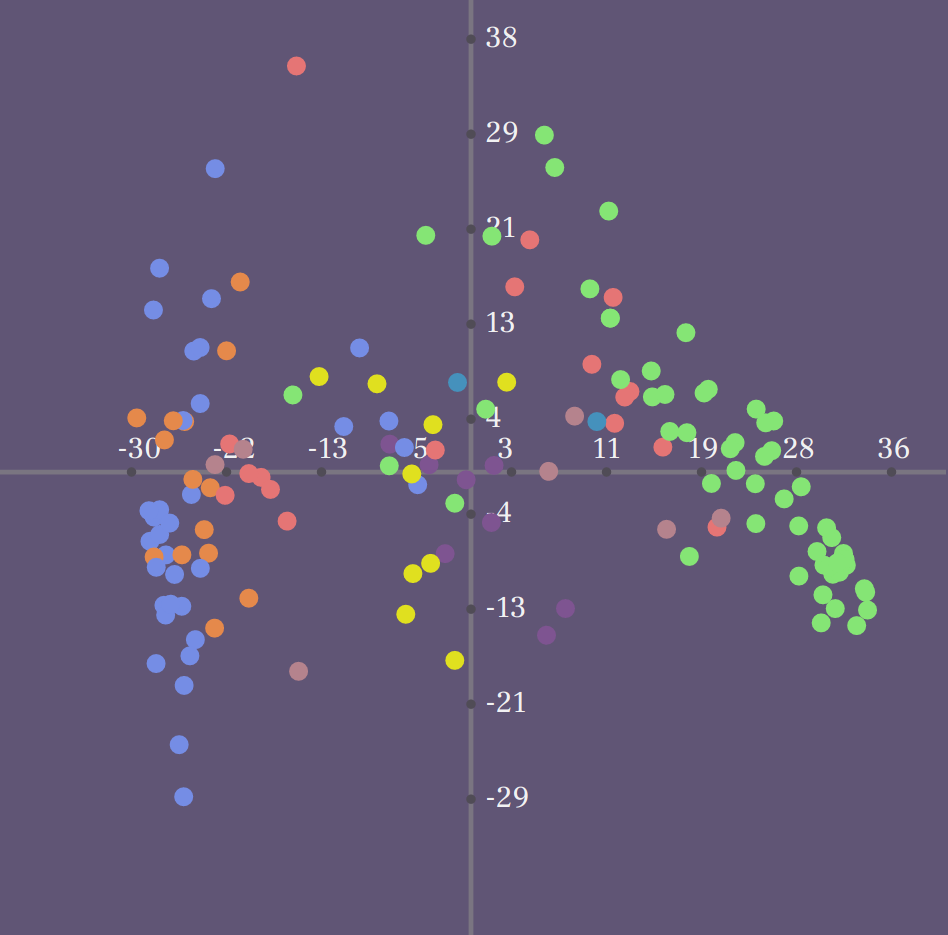
\includegraphics[width=0.46\textwidth]{images/mds}\label{fig:majority_vs_minority_k3_actual}}
	\caption{majority vs minority, k=3, \gls{k-means} on \acrshort{mds} coordinates}
\end{figure}

	\clearpage


	
	\subsubsection{Secret groups}
	
	There are 8 factions in current term of office. 8th faction is mixed group, meaning they will not vote in unison. In perfect scenario remaining 7 factions should be classified by classifier. To see how differently voting patterns can group - one group with less than 7 clusters should be tried and another one with more than 8 to see how well it matches current factions.

   	
   		\noindent
   	\begin{center}
   		\begin{tabular}{L{3cm} C{2cm} C{2cm} C{2cm}}
   			\multicolumn{2}{c}{}\\ 
   			\hline
   			Encoding & k=7 & k=8 & k=9 \\\hline
   			E1 & 446888 & 432739 & 428739 \\
   			E2 & 100255 & 99660 & 98591 \\
   			E3 & 706380 & 694879 & 688514 \\
   			
   			\hline
   		\end{tabular}
   		\captionof{table}{ Distortion for \gls{k-means} secret groups results} \label{tab:k_means_performance_secret}
   	\end{center} 
   
   \begin{figure}[!tbp]
   	\centering
   	\subfloat[k=7, encoding = E1]{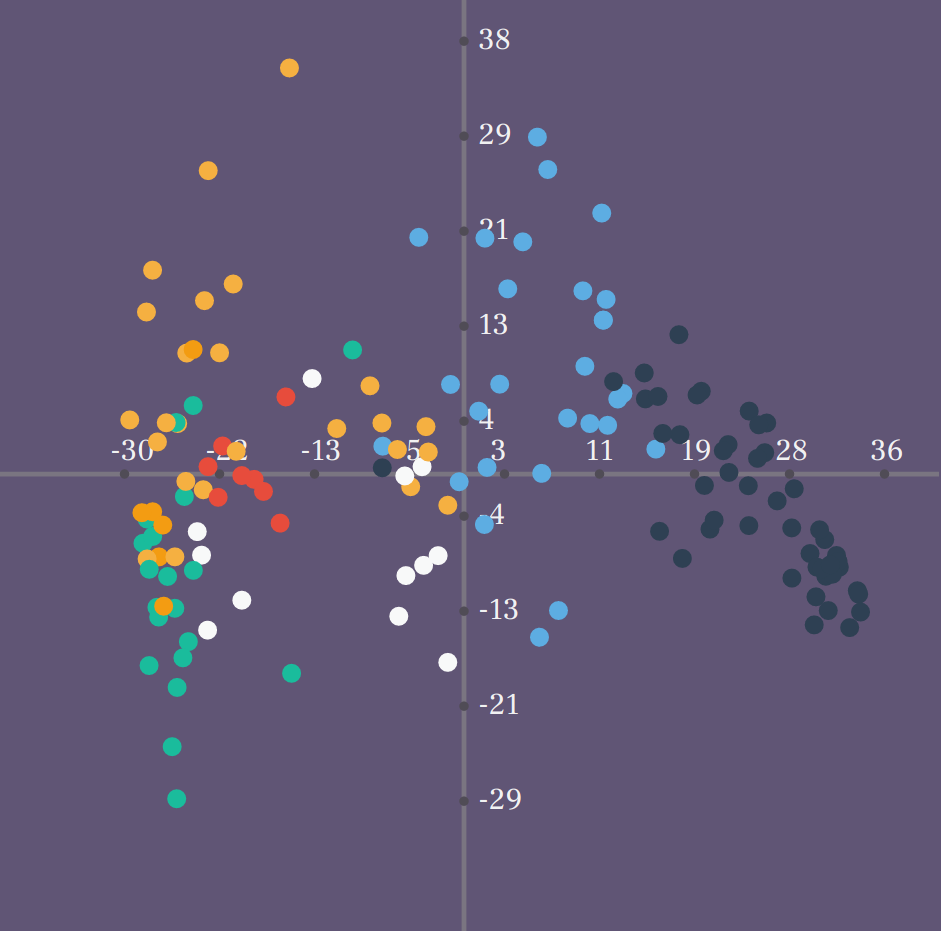
\includegraphics[width=0.46\textwidth]{images/kmeans_k7_e1}\label{fig:secret_groups_k7_e1}}
   	\hfill
   	\subfloat[k=7, encoding = E2]{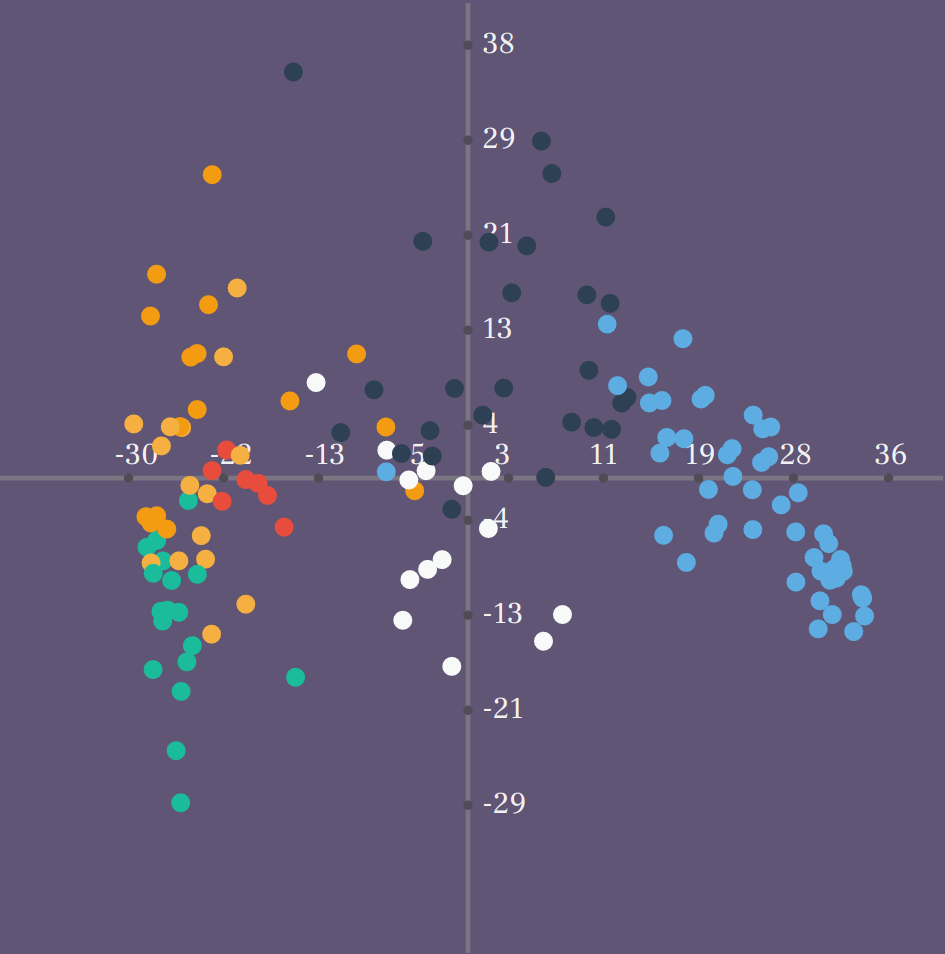
\includegraphics[width=0.46\textwidth]{images/kmeans_k7_e2}\label{fig:secret_groups_k7_e2}}
   	\hfill
   	\subfloat[k=7, encoding = E3]{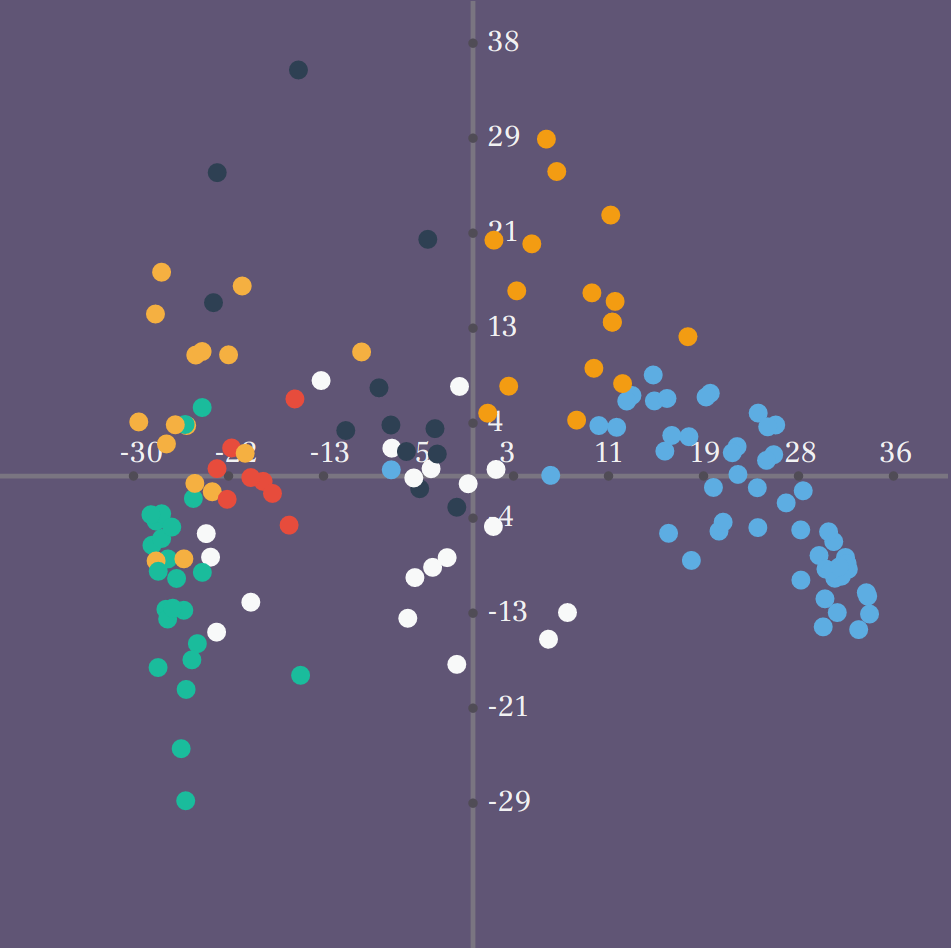
\includegraphics[width=0.46\textwidth]{images/kmeans_k7_e3}\label{fig:secret_groups_k7_e3}}
   	\hfill
	\subfloat[Actual factions]{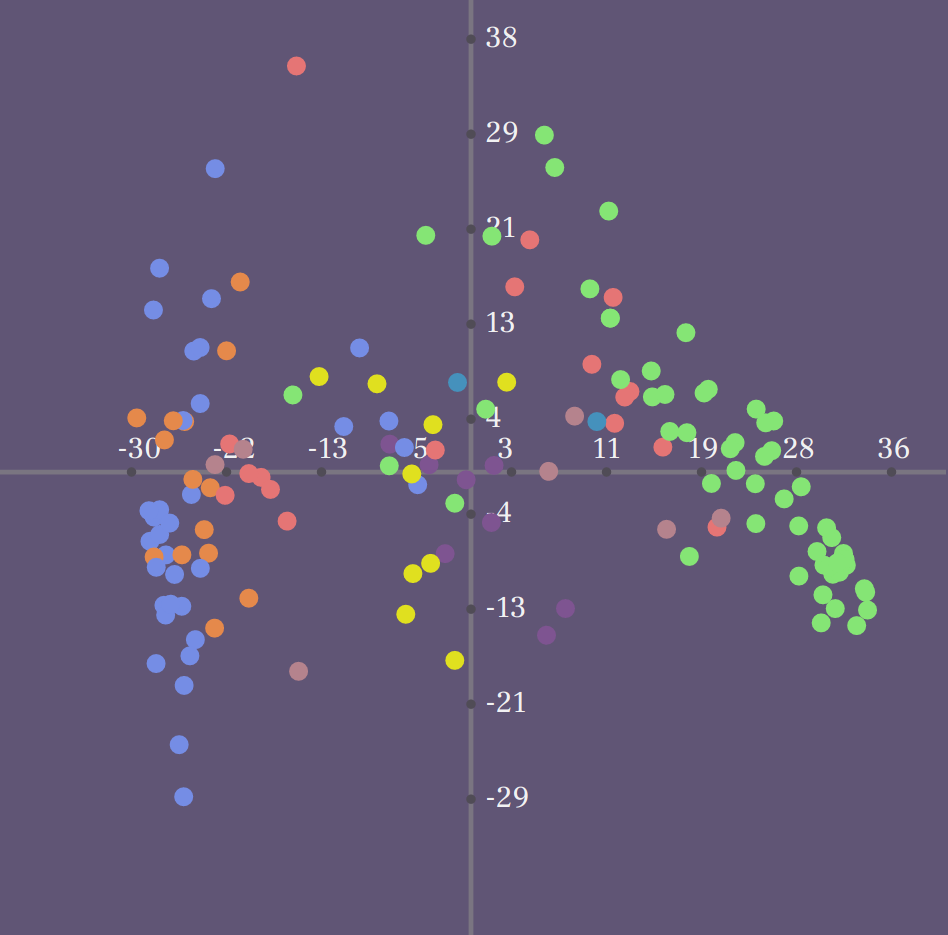
\includegraphics[width=0.46\textwidth]{images/mds}\label{fig:majority_vs_minority_actual}}
   	\caption{different clusters of members, \gls{k-means} on \acrshort{mds} coordinates}
   \end{figure}
   
   \clearpage
   
   \begin{figure}[!tbp]
   	\centering
   	\subfloat[k=8, encoding = E1]{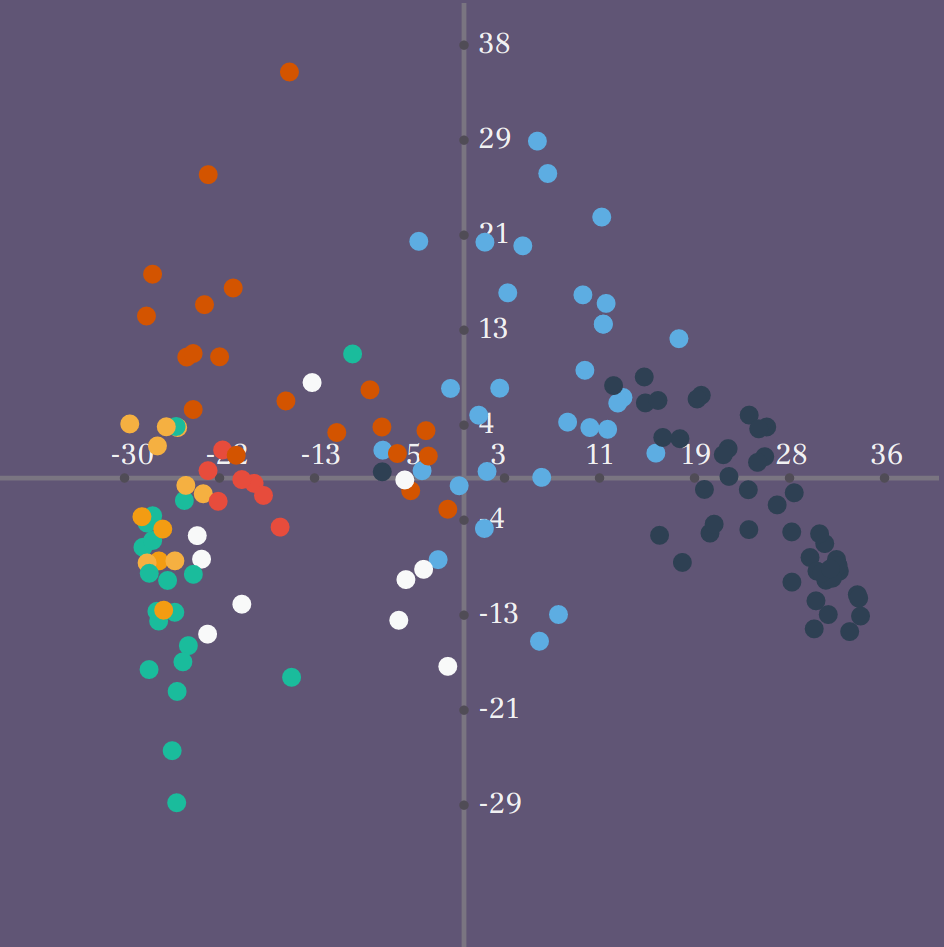
\includegraphics[width=0.46\textwidth]{images/kmeans_k8_e1}\label{fig:secret_groups_k8_e1}}
   	\hfill
   	\subfloat[k=8, encoding = E2]{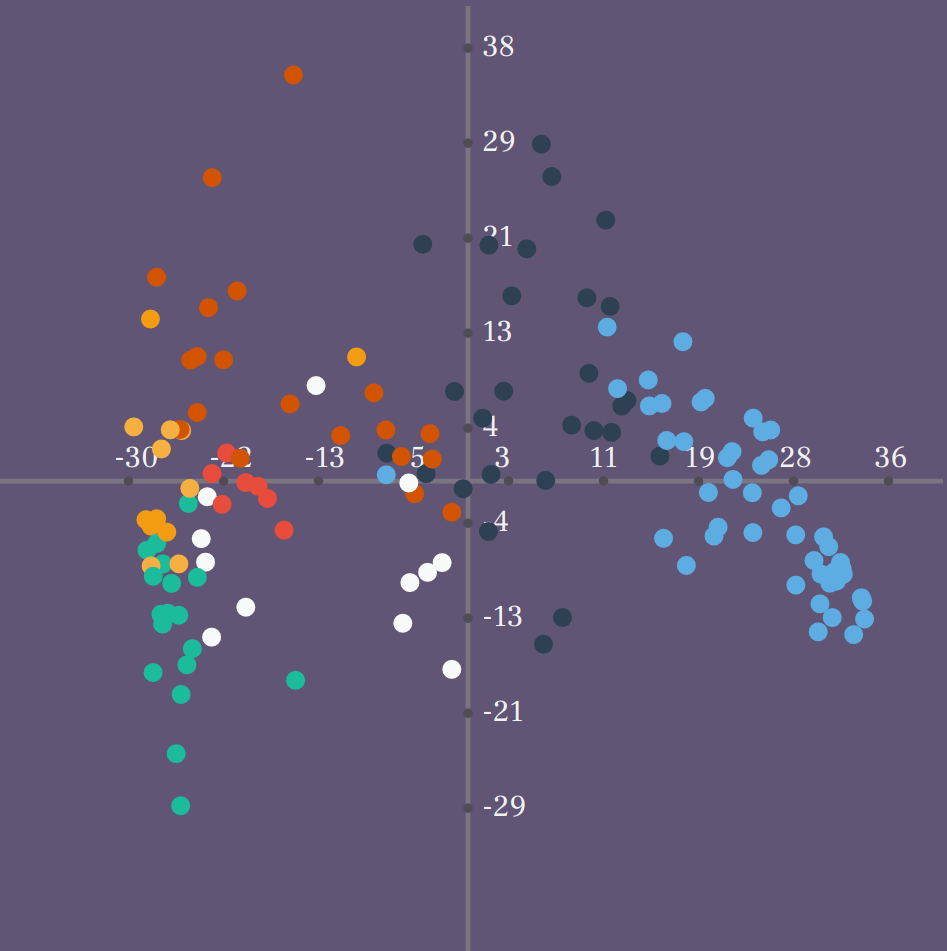
\includegraphics[width=0.46\textwidth]{images/kmeans_k8_e2}\label{fig:secret_groups_k8_e2}}
   	\hfill
   	\subfloat[k=8, encoding = E3]{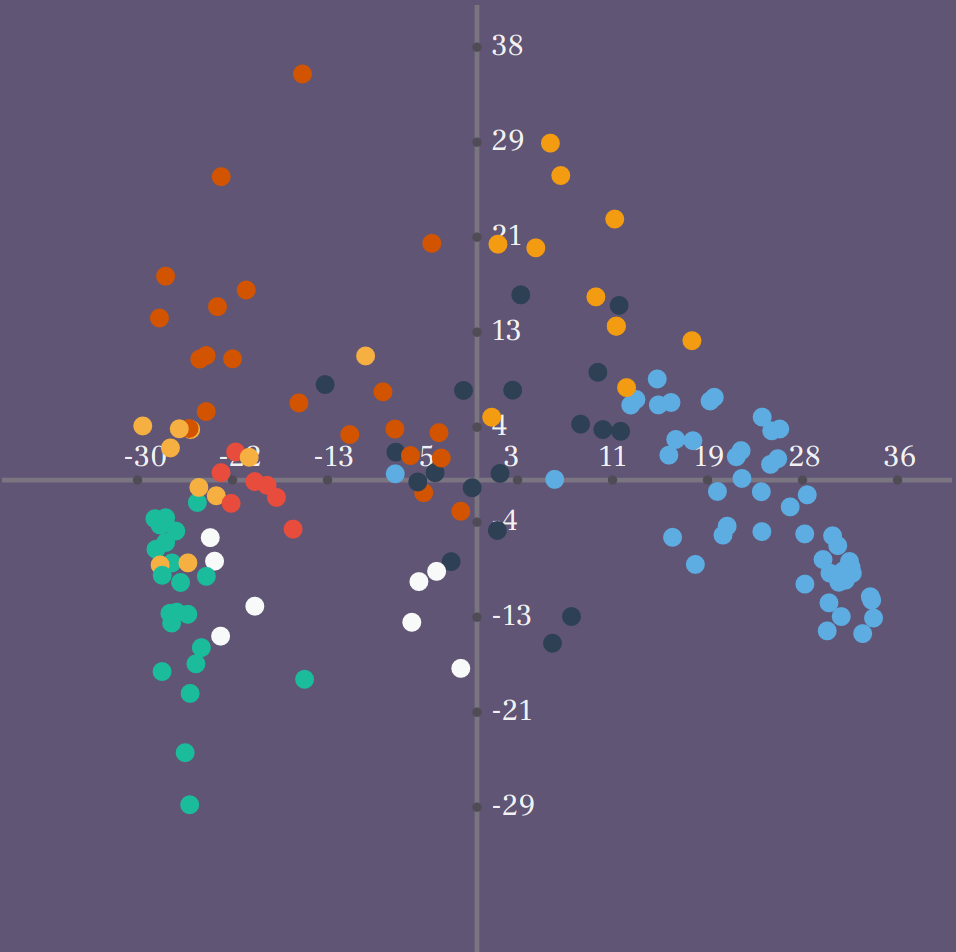
\includegraphics[width=0.46\textwidth]{images/kmeans_k8_e3}\label{fig:secret_groups_k8_e3}}
   	\caption{different clusters of members, \gls{k-means} on \acrshort{mds} coordinates}
   \end{figure}
   
   \clearpage
   
     \begin{figure}[!tbp]
   	\centering
   	\subfloat[k=9, encoding = E1]{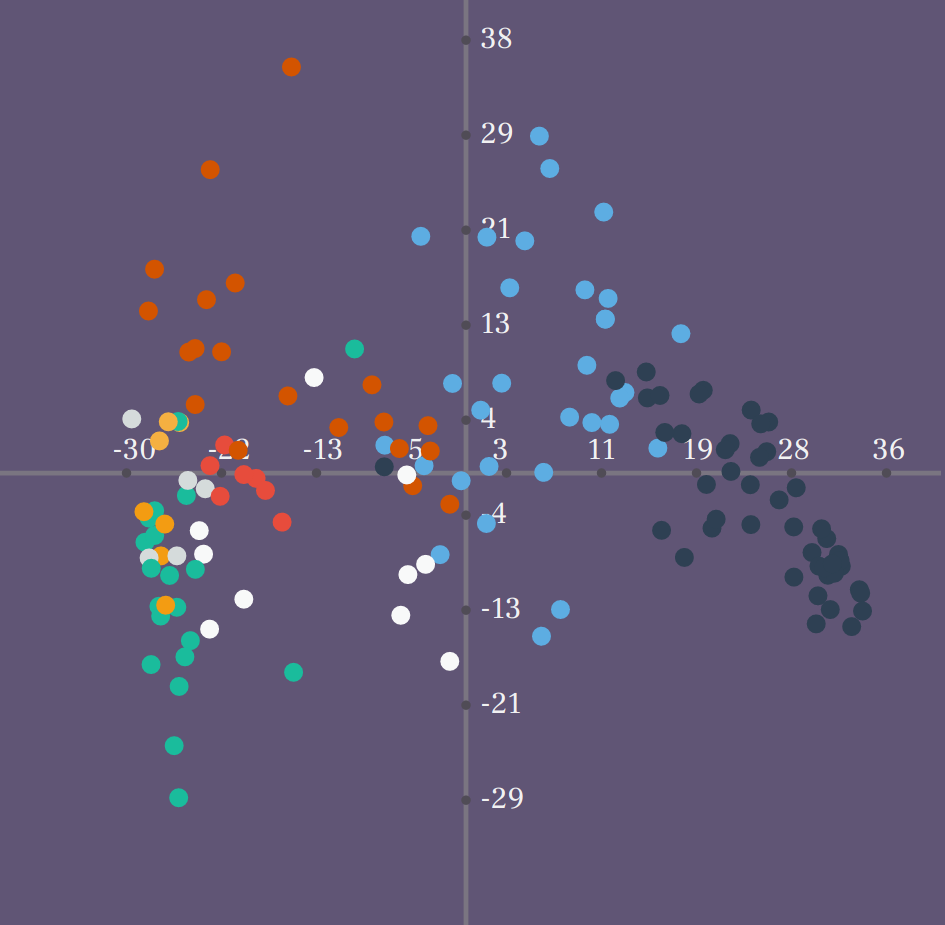
\includegraphics[width=0.46\textwidth]{images/kmeans_k9_e1}\label{fig:secret_groups_k9_e1}}
   	\hfill
   	\subfloat[k=9, encoding = E2]{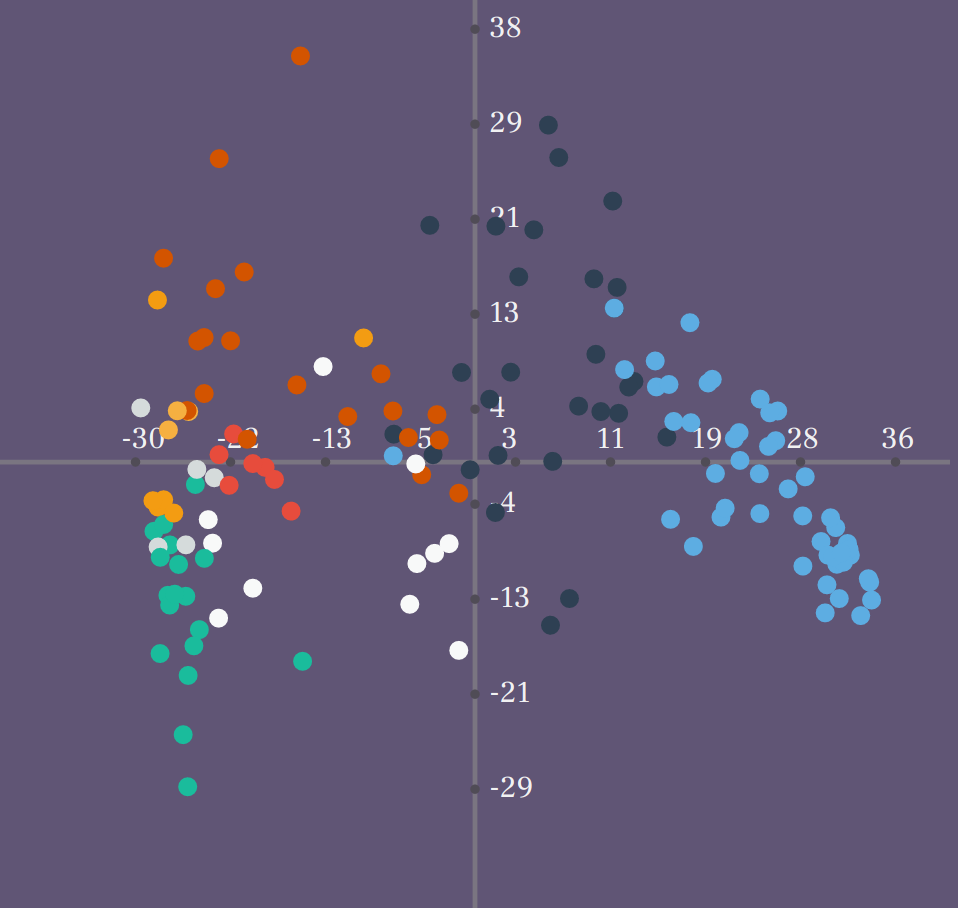
\includegraphics[width=0.46\textwidth]{images/kmeans_k9_e2}\label{fig:secret_groups_k9_e2}}
   	\hfill
   	\subfloat[k=9, encoding = E3]{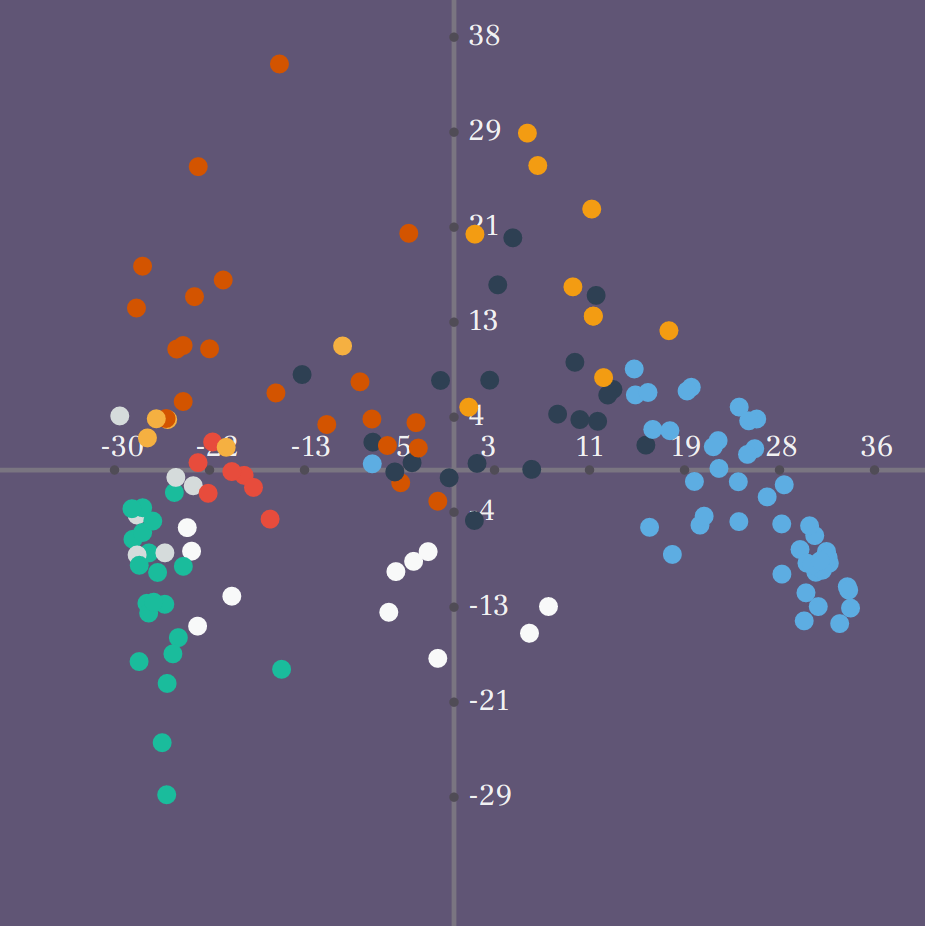
\includegraphics[width=0.46\textwidth]{images/kmeans_k9_e3}\label{fig:secret_groups_k9_e3}}
   	\caption{different clusters of members, \gls{k-means} on \acrshort{mds} coordinates}
   \end{figure}
   
   \clearpage
   	
   	\subsection{Results and conclusions}
    
   
    \clearpage
    
    \bibliography{bibtex}{}
    \bibliographystyle{ieeetr}
        
    \clearpage
    
    \pagenumbering{roman}
      
	\appendix
	\section{Appendix}
    
    \end{document}